
\documentclass[gr]{cseuoi-thesis} % Διπλωματική εργασία (στα Ελληνικά)

\titleGr{Τοπολογία και συγχρονισμός στο OpenMP για συστήματα NUMA πάρα πολλών πυρήνων}
\titleEn{Topology and synchronization in OpenMP for NUMA manycore systems}
\authorGr{Γεώργιος Ζ. Ζάχος}
\authorEn{Georgios Z. Zachos}
\aitiatiki{Γεώργιο Ζ. Ζάχο}
\dateGr{Σεπτέμβριος 2021}
\dateEn{September 2021}
\advisorGr{Βασίλειος Β. Δημακόπουλος, Αναπληρωτής Καθηγητής}
\advisorEn{Vassilios V. Dimakopoulos, Associate Professor}

% Πακέτο για την εμφάνιση περιθωρίων (χρήσιμο για την εύρεση overfull boxes)
%\usepackage{showframe}

% Πακέτο για τη διατήρηση των floats (εικόνες κ.α.) εντός των ενοτήτων
\usepackage[section]{placeins}

%
\usepackage{listings}
\usepackage{tablefootnote}

\lstset{
	language=C,
	numbers=left,
	basicstyle=\footnotesize\ttfamily,
	commentstyle=\itshape\color{gray},
	numberstyle=\scriptsize,
	numbersep=12pt,
	tabsize=4,
	extendedchars=true,
	breaklines=true,
	frame=b,
	xleftmargin=24pt,
	framexleftmargin=24pt,
	framexrightmargin=2pt
}

\usepackage{caption}
\DeclareCaptionFont{white}{\color{white}}
\DeclareCaptionFormat{listing}{\colorbox[cmyk]{0.43, 0.35, 0.35, 0.01}{\parbox{\textwidth}{\hspace{15pt}#1#2#3}}}
\captionsetup[lstlisting]{format=listing,labelfont=white,textfont=white, singlelinecheck=false, margin=0pt, font={bf,footnotesize}}

\renewcommand\lstlistingname{Πρόγραμμα}
\renewcommand\lstlistlistingname{Κατάλογος Προγραμμάτων}

\begin{document}

% Σελίδες χωρίς αρίθμηση
\pagenumbering{gobble}

% Εκτύπωση της σελίδας τίτλου
\maketitle

% Αρχικοποίηση του minitoc
\dominitoc[n]

\chapter*{\cseafierwsi}

Η σελίδα αυτή είναι προαιρετική και περιέχει αφιέρωση σε κάποιο σημαντικό πρόσωπο.

\bigskip

\noindent Προτεινόμενο: 1-2 γραμμές.

\noindent Μέγιστο: 1 σελίδα.
 % Προαιρετικό
% \chapter*{\cseeuxaristies}

Η σελίδα αυτή είναι προαιρετική και περιέχει ευχαριστίες σε άτομα που βοήθησαν με οποιονδήποτε τρόπο τον συγγραφέα της διατριβής.

\bigskip

\noindent Προτεινόμενο: 10-15 γραμμές.

\noindent Μέγιστο: 1 σελίδα. % Προαιρετικό


% Σελίδες με αρίθμηση i, ii, iii, iv, ...
\pagenumbering{roman}

% Περιεχόμενα
\pdfbookmark{\contentsname}{contents} % hyperref
\tableofcontents

% Κατάλογος Σχημάτων
\addstarredchapterc{\listfigurename} % minitoc
\listoffigures

% Κατάλογος Πινάκων
\addstarredchapterc{\listtablename} % minitoc
\listoftables

% Κατάλογος Προγραμμάτων
\addstarredchapterc{\lstlistingname} % minitoc
\lstlistoflistings

% Κατάλογος Αλγορίθμων
%\addstarredchapterc{\listalgorithmname} % minitoc
%\listof{algorithm}{\listalgorithmname}

% \chapter*{\glossaryname}
% Εισαγωγή του κεφάλαιου στα περιεχόμενα
\addstarredchapter{\glossaryname} %minitoc

Η σελίδα αυτή είναι προαιρετική.
Περιέχει ορισμούς και επεξηγήσεις εννοιών, όρων, συντομεύσεων, και συμβολισμών.
Αν η έκτασή τους είναι μεγαλύτερη από δύο σελίδες τότε πρέπει να πάει στο τέλος της διπλωματικής εργασίας, αμέσως μετά τα παραρτήματα. % Προαιρετικό

% Περίληψη στη γλώσσα συγγραφής (π.χ. Ελληνικά)
\chapter*{\abstractname}
\addstarredchapter{\abstractname} % minitoc
\makecseabstract


\noindent Η ολοένα και αυξανόμενη ανάγκη για μεγαλύτερη επεξεργαστική ισχύ οδήγησε στη δημιουργία των συστημάτων \textit{μη ομοιόμορφης προσπέλασης μνήμης} (NUMA) τα οποία αποτελούν αρχιτεκτονική εξέλιξη των κοινών \textit{συμμετρικών πολυεπεξεργαστών} (SMPs) και τα οποία είναι εφοδιασμένα με μεγάλους αριθμούς επεξεργαστικών πυρήνων. Τα συστήματα αυτά παρέχουν κοινόχρηστο χώρο διευθύνσεων και συνεπώς επιτρέπουν την ανάπτυξη προγραμμάτων με διαδεδομένες \textit{διεπαφές προγραμματισμού εφαρμογών} (APIs) όπως το OpenMP. Λόγω της πολύπλοκης αρχιτεκτονικής οργάνωσης των συστημάτων NUMA, η επίτευξη των βέλτιστων δυνατών επιδόσεων συνήθως απαιτεί την εκμετάλλευση πληροφοριών που σχετίζονται με την τοπολογία του υποκείμενου συστήματος, δηλαδή με το πώς είναι οργανωμένο το υλικό. Ήδη από την έκδοση 4.0 του OpenMP, άρχισαν να προδιαγράφονται λειτουργίες όπως τα OpenMP places και OpenMP processor binding policies οι οποίες σχετίζονται με την τοπολογία και επιτρέπουν στο χρήστη να ελέγξει τον τρόπο ανάθεσης των νημάτων στα διαθέσιμα επεξεργαστικά στοιχεία. Στα πλαίσια της παρούσας διπλωματικής εργασίας, θα ασχοληθούμε με την υλοποίηση των λειτουργιών OpenMP places και OpenMP processor binding policies, καθώς επίσης θα προσπαθήσουμε να βελτιώσουμε τις υπάρχουσες λειτουργίες συγχρονισμού, όπως οι \textit{κλήσεις φραγής} (barriers), ώστε να λειτουργούν αποδοτικά σε συστήματα NUMA.


\bigskip

% Περίληψη στην αντίθετη γλώσσα από τη γλώσσα συγγραφής (π.χ. Αγγλικά)
\chapter*{\csebilabstract}
\addstarredchapter{\csebilabstract} % minitoc
\makecsebilabstract

\noindent The growing need for more processing power has led to the proliferation of \textit{non-uniform memory access} (NUMA) systems which constitute the architectural evolution of \textit{symmetric multiprocessors} (SMPs) and can be equipped with a large number of processing cores. These systems provide a shared-address space and therefore can be programmed %allow the development of programs
using widespread \textit{application programming interfaces} (APIs) such as the OpenMP API. Due to the complex architectural organization of NUMA systems, achieving the best possible performance usually requires using information related to the topology of the underlying system, that is, information about how its hardware is organized. Since version 4.0 of the OpenMP specification, topology-related features such as \textit{OpenMP places} and \textit{OpenMP processor binding policies} have beed introduced in order to allow users to control the assignment of threads to the available processing elements. In the context of this diploma thesis, the OpenMP places and OpenMP processor binding policies primitives were fully implemented. In addition, synchronization functions, specifically barriers, were redesigned to function efficiently on large NUMA systems.

\bigskip



% Σελίδες με αρίθμηση 1, 2, 3, 4, ...
\pagenumbering{arabic}

% Εισαγωγή των κεφαλαίων
\chapter{Εισαγωγή}
\label{ch:Introduction}

\section{Η ανάγκη για παράλληλα συστήματα} % Η εξέλιξη των σύγχρονων Η/Υ
\label{sec:The need for parallel systems}
Η βασική ιδέα της οργάνωσης των ηλεκτρονικών υπολογιστών με τη μορφή που αυτοί είναι γνωστοί έως και σήμερα, βασίζεται στην αρχιτεκτονική von Neumann όπως αυτή περιγράφηκε το 1945 από τον ουγγρικής και αμερικανικής καταγωγής μαθηματικό John von Neumann. Βάσει αυτής της περιγραφής, υπάρχει μία μονάδα επεξεργασίας η οποία επικοινωνεί με το τμήμα μνήμης, εκτελώντας εντολές και τροποποιώντας δεδομένα. Ο επεξεργαστής λαμβάνει μία-μία τις εντολές από τη μνήμη και τις εκτελεί προσπελαύνοντας ή/και τροποιοιώντας δεδομένα που βρίσκονται στη μνήμη όταν αυτό καθορίζεται από την εντολή, με αυτό τον κύκλο να επαναλαμβάνεται συνεχώς. Το μοντέλο προγραμματισμού που χρησιμοποιείται στη συγκεκριμένη αρχιτεκτονική είναι γνωστό και ως σειριακό μοντέλο και φαίνεται στο Σχήμα X.

Η εποχή της πληροφορίας που ξεκίνησε στα μέσα του 20\textsuperscript{ού} αιώνα και οδήγησε σε μία οικονομία βασισμένη στην τεχνολογία της πληροφορίας, καθώς και η ολοένα και μεγαλύτερη χρήση των Η/Υ σε κάθε πτυχή της ζωής του ανθρώπου είχαν ως αποτέλεσμα την έναρξη ενός αγώνα ταχύτητας με σκοπό την κατασκευή όλο και πιο γρήγορων υπολογιστών.

Η κλιμάκωση της συχνότητας (frequency scaling) που αφορά την αύξηση της συχνότητας ενός επεξεργαστή με στόχο την επίτευξη μεγαλύτερης επίδοσης στα συστήματα που τον χρησιμοποιούν, αποτέλεσε τον κύριο λόγο αύξησης των επιδόσεων των εμπορικών Η/Υ από τα μέσα του 1980 έως και περίπου τα τέλη του 2004, όταν αυτή η προσπάθεια προσέκρουσε στο τείχος της ισχύος (power wall) όπως φαίνεται στο Σχήμα Χ. Αυτό συνέβει καθώς η αύξηση της συχνότητας οδήγησε στην αύξηση της καταναλισκόμενης ισχύος η οποία με τη σειρά της είχες ως αποτέλεσμα την αύξηση του κόστους λειτουργίας αλλά και την οδήγηση του υλικού στα όριά του με χαρακτηριστικό παράδειγμα την υπερθέρμανσή του.

%Η κλιμάκωση της συχνότητας (frequency scaling) αφορά την αύξηση της συχνότητας ενός επεξεργαστή με στόχο την επίτευξη μεγαλύτερης επίδοσης στα συστήματα που χρησιμοποιούν αυτόν τον επεξεργαστή. Η κλιμάκωση της συχνότητας αποτέλεσε την κινητήριο δύναμη που οδήγησε στην αύξηση των επιδόσεων των εμπορικών Η/Υ από τα μέσα του 1980 έως και περίπου τα τέλη του 2004, μέχρις ότου αυτή η προσπάθεια προσέκρουσε στο τείχος της ισχύος (power wall). Αυτό συνέβει καθώς η αύξηση της συχνότητας οδήγησε στην αύξηση της καταναλισκόμενης ισχύος η οποία με τη σειρά της οδήγησε σε μεγάλη κατανάλωση ρεύματος και υπερθέρμανση του υλικού.

Για να ξεπεραστεί το τείχος της ισχύος, οι κατασκευαστές των επεξεργαστών άρχισαν να ενσωματώνουν παραπάνω του ενός επεξεργαστικούς πυρήνες στο ίδιο ολοκληρωμένο κύκλωμα επεξεργαστή. Η αρχιτεκτονική αυτή βελτίωση είχε ως αποτέλεσμα τη γέννηση των πρώτων πολυπύρηνων επεξεργαστών οι οποία έκαναν δυνατή την ταυτόχρονη εκτέλεση εντολών. Τα συστήματα που περιείχαν πολυπύρηνους επεξεργαστές αποτέλεσαν τα πρώτα εμπορικά μικρού μεγέθους παράλληλα συστήματα.

Στη σημερινή εποχή, τα πολυπύρηνα συστήματα είναι ευρέως διαδεδομένα καθώς απαντώνται από κινητά τηλέφωνα και ενσωματωμένους υπολογιστές χαμηλού κόστους και μεγέθους όσο μια πιστωτική κάρτα τραπέζης, μέχρι και υπολογιστικά συστήματα πολύ υψηλών επιδόσεων που διεξάγουν επιστημονικούς υπολογισμούς.


\section{Κατηγορίες Παράλληλων Συστημάτων}
\label{sec:Parallel System Categories}
Όταν μιλάμε για παράλληλα συστήματα ουσιαστικά αναφερόμαστε σε συστήματα με μία συλλογή από επεξεργαστικές μονάδες που επικοινωνούν και συνεργάζονται για τη λύση ενός προβλήματος. Το πρόβλημα χωρίζεται σε επιμέρους εργασίες οι οποίες με τη σειρά τους ανατίθενται στις επεξεργαστικές μονάδες για εκτέλεση. Παρόλο που η ιδέα των πολλαπλών επεξεργαστικών μονάδων φαίνεται απλή, προκύπτουν ζητήματα τα οποία σχετίζονται πλην άλλων με τον τρόπο:
\begin{itemize}
	\item επικοινωνίας, συγχρονισμού και συντονισμού των επεξεργαστικών μονάδων
	\item διαμοιρασμού των εργασιών και
	\item προγραμματισμού ανάλογα με την οργάνωση του εκάστοτε συστήματος.
\end{itemize}
 
\subsection{Ταξινομία του Flynn}
Μία αρχική κατηγοριοποίηση των παράλληλων συστημάτων μπορεί να γίνει βάσει της ταξινομίας του Flynn και η οποία περιλαμβάνει τις εξής κατηγορίες:
\begin{itemize}
	\item SISD (single-instruction single-data) Σχήμα Χ
	\item SIMD (single-instruction multiple-data) Σχήμα Χ και
	\item MIMD (mutiple-instruction multiple-data) Σχήμα Χ
\end{itemize}

Στην κατηγορία SISD ανήκουν οι κλασικοί σειριακοί υπολογιστές οι οποίοι εκτελούν μία εντολή τη φορά (single-instruction) επάνω σε ένα δεδομένο (single-data). Στην κατηγορία SIMD συναντάμε επίσης υπολογιστές οι οποίοι εκτελούν μία εντολή τη φορά, αλλά μπορούν να την εφαρμόσουν ταυτόχρονα σε πολλαπλά δεδομένα (multiple-data) ώστε να εκμεταλλευτούν την παραλληλία επιπέδου δεδομένων (data-level parallelism). Τέλος, η κατηγορία MIMD θεωρείται ως η κατηγορία των καθαρά παράλληλων υπολογιστών οι οποίοι μπορούν και εκτελούν ταυτόχρονα πολλαπλές εντολές, με κάθε μία να ασχολείται με διαφορετικό δεδομένο.

Όπως θα δούμε στη συνέχεια, οι υπολογιστές MIMD, μπορούν να κατηγοριοποιηθούν περαιτέρω βάσει του πώς είναι οργανωμένη η μνήμη τους.

\subsection{Ταξινόμηση βάσει της οργάνωσης της μνήμης}
Η ταξινόμηση των παράλληλων υπολογιστών σχετικά με το πώς είναι οργανωμένη η μνήμη μπορεί να γίνει είτε βάσει της φυσικής οργάνωσης της μνήμης είτε βάσει της εικόνας/άποψης που έχει ο προγραμματιστής για αυτή.

Σχετικά με την πρώτη κατηγοριοποίηση, οι παράλληλοι υπολογιστές διακρίνονται σε υπολογιστές με (φυσικά) κοινόχρηστη μνήμη (γνωστοί και ως πολυεπεξεργαστές) και σε υπολογιστές με (φυσικά) κατανεμημένη μνήμη.

Όσον αφορά την εικόνα που έχει ο προγραμματιστής για την οργάνωση της μνήμης, οι υπολογιστές μπορούν να διαχωριστούν σε υπολογιστές με κοινόχρηστο και σε υπολογιστές με κατανεμημένο χώρο διευθύνσεων. Αξίζει να σημειωθεί ότι η εικόνα από προγραμματιστική άποψη δεν ταυτίζεται απαραίτητα με την φυσική οργάνωση της μνήμης καθώς με χρήση ειδικού λογισμικού ένα σύστημα με φυσικά κατανεμημένη μνήμη μπορεί να παρέχει κοινόχρηστο χώρο διευθύνσεων.


\subsubsection{Συστήματα κοινόχρηστης μνήμης}
Τα συστήματα κοινόχρηστης μνήμης (SMM - Shared Memory Machines *bib*) αποτελούνται από επεξεργαστές, κοινόχρηστη μνήμη (γνωστή και ως καθολική) η οποία είναι καθολικά προσβάσιμη από όλους τους επεξεργαστές και ένα δίκτυο διασύνδεσης για την επικοινωνία των επεξεργαστών με τη μνήμη. Από άποψη φυσικής οργάνωσης, η μνήμη μπορεί να αποτελείται από περισσότερα του ενός τμήματα/μέρη (modules) τα οποία όμως παρέχουν έναν κοινόχρηστο χώρο διευθύνσεων που είναι προσβάσιμος από όλους τους επεξεργαστές. Οι επεξεργαστές επικοινωνούν, συνεργάζονται και ανταλλάσσουν δεδομένα διαβάζοντας ή γράφοντας σε κοινόχρηστες μεταβλητές που βρίσκονται αποθηκευμένες στη μνήμη.

Το δίκτυο διασύνδεσης επεξεργαστών-μνήμης μπορεί να είναι ένας απλός δίαυλος (bus), ένα διακοπτικό δίκτυο (π.χ. crossbar) ή κάποιο δίκτυο πολλαπλών επιπέδων (π.χ. Δίκτυο Δέλτα). Στην περίπτωση που το δίκτυο διασύνδεσης είναι δίαυλος, τότε αναφερόμαστε σε αυτά τα συστήματα ως Συμμετρικοί Πολυεπεξεργαστές (SMPs - Symmetric Multiprocessors). Οι Συμμετρικοί Πολεπεξεργαστές διαθέτουν μία κοινόχρηστη μνήμη η οποία απέχει εξίσου από όλους τους επεξεργαστές και συνεπώς χαρακτηρίζονται ως συστήματα ομοιόμορφης προσπέλασης μνήμης (UMA - Uniform Memory Access). Όπως είναι φυσικό, αν οι επεξεργαστές είναι πολυπύρηνοι και διαθέτουν ιεραρχία από πολύ μικρές αλλά ταυτόχρονα πολύ γρήγορες μνήμες γνωστές ως κρυφές μνήμες (caches), τότε ο κάθε πολυπύρηνος επεξεργαστής αποτελεί ένα σύστημα SMP καθώς η πρόσβαση στην κρυφή μνήμη είναι πιο γρήγορη από την πρόσβαση στην κύρια μνήμη μέσω του διαύλου.

Επειδή το εύρος ζώνης (bandwidth) του διαύλου είναι σταθερό ανεξάρτητα από το πλήθος των επεξεργαστών που είναι συνδεδεμένοι σε αυτόν, όσο πιο πολλοί επεξεργαστές είναι συνδεδεμένοι, τόσο πιο πολύ υποβαθμίζεται η αποδοτικότητα του δικτύου λόγω των συγγρούσεων πρόσβασης στο κοινό μέσο και συνεπώς τόσο περισσότερο καθυστερεί η εξυπηρέτηση προσπελάσεων στη μνήμη. Για την αποδοτική υποστήριξη μεγαλύτερου αριθμού επεξεργαστών καταφεύγουμε στη χρήση κρυφής μνήμης ή άλλου τύπου δίκτυου διασύνδεσης.

Παράλληλα συστήματα μεγαλύτερου μεγέθους μπορούν να υλοποιηθούν χρησιμοποιώντας Συμμετρικούς Πολυεπεξεργαστές ως κόμβους ενός δικτύου διασύνδεσης (Σχήμα Χ). Σε αυτά τα συστήματα καθίσταται δυνατή η παροχή ενός κοινόχρηστου χώρου διευθύνσεων με χρήση κατάλληλων πρωτοκόλλων συνοχής τα οποία αποκρύπτουν από τον χρήστη του συστήματος την κατανεμημένη οργάνωση της φυσικής μνήμης. Η αρχιτεκτονική που μόλις περιγράφηκε είναι γνωστή και ως κατανεμημένη κοινόχρηστη μνήμη (DSM - Distrubuted Shared Memory), ενώ τα συστήματα αυτά ονομάζονται συστήματα ανομοιόμορφης προσπέλασης μνήμης (NUMA - Non-Uniform Memory Access). Σε περίπτωση ύπαρξης ιεραρχίας κρυφών μνημών στους κόμβους (Σχήμα Χ), χρειάζεται η χρήση ενός πρωτοκόλλου συνοχής κρυφής μνήμης (cache coherence protocol) το οποίο θα εξασφαλίζει ανά πάσα στιγμή ότι οποιαδήποτε προσπέλαση μνήμης θα επιστρέφει την πιο πρόσφατη τιμή. Τέτοια συστήματα είναι γνωστά ως cc-NUMA (Cache coherent NUMA).

\subsubsection{Συστήματα κατανεμημένης μνήμης}
Τα συστήματα κατανεμημένης μνήμης (DMM - Distributed Memory Machines) αποτελούνται από επεξεργαστικά στοιχεία (γνωστά και ως κόμβοι) και από ένα δίκτυο διασύνδεσης το οποίο επιτρέπει την επικοινωνία μεταξύ των κόμβων (Σχήμα Χ) *ref*. Κάθε κόμβος περιέχει επεξεργαστή, τοπική μνήμη και ίσως περιφερειακές συσκευές. Η τοπική μνήμη κάθε κόμβου είναι απευθείας προσβάσιμη μόνο από τον επεξεργαστή του ίδιου κόμβου, ενώ όταν κάποιος επεξεργαστής χρειάζεται να προσπελάσει την τοπική μνήμη που βρίσκεται σε κάποιον άλλο κόμβο, αυτό επιτυγχάνεται με τη μεταβίβαση μηνυμάτων μέσω του δικτύου διασύνδεσης. 

Συλλογές υπολογιστών που είναι συνδεδεμένοι μέσω δικτύου διασύνδεσης αφιερωμένου αποκλειστικά στη μεταξύ τους επικοινωνία ονομάζονται συστάδες (clusters). Οι συστάδες υπολογιστών χρησιμοποιούνται ευρέως λόγω της διαθεσιμότητας δικτύων διασύνδεσης υψηλών επιδόσεων όπως το Switched Gigabit Ethernet, το Infiniband, το Myriret κ.ά. Πολλαπλές συστάδες υπολογιστών μπορούν να διασυνδεθούν μεταξύ τους και να δημιουργήσουν συστήματα πλέγματος (grids).

Το πλήθος των κόμβων και αντίστοιχα το πλήθος των επεξεργαστών στα συστήματα κατανεμημένης μνήμης μπορεί να φτάσει τις δεκάδες χιλιάδες, σε αντίθεση με τα συστήματα κοινόχρησης μνήμης όπου το πλήθος των επεξεργαστών περιορίζεται σε μερικές δεκάδες. Προφανώς, η ικανότητα κλιμάκωσης των κατανεμημένων συστημάτων εξαρτάται από την σωστή επιλογής της τοπολογίας του δικτύου διασύνδεσης.


\section{Προγραμματισμός Παράλληλων Συστημάτων}

\subsection{Συστήματα κοινόχρηστης μνήμης}
Ο προγραμματισμός των συστημάτων κοινόχρηστης μνήμης συνήθως βασίζεται στη χρήση νημάτων, δηλαδή ξεχωριστές ακολουθίες ελέγχου (στοίβα + μετρητής προγράμματος) που μοιράζονται δεδομένα με τα υπόλοιπα άλλα νήματα μέσω κοινόχρηστου χώρου διευθύνσεων. Η ύπαρξη κοινόχρηστων δεδομένων εγείρει ζητήματα όπως αυτό της ταυτόχρονης προσπέλασής τους από διαφορετικά νήματα, καθώς κάτι τέτοιο θα μπορούσε να οδηγήσει σε συνθήκες ανταγωνισμού (race conditions). Όταν υπάρχουν συνθήκες ανταγωνισμού, το τελικό αποτέλεσμα των ταυτόχρονων προσπελάσεων μνήμης εξαρτάται από τις σχετικές ταχύτητες εκτέλεσεις των νημάτων. Για την αποφυγή συνθηκών ανταγωνισμού και την εξασφάλιση της ακεραιότητας των δεδομένων χρησιμοποιείται ο αμοιβαίος αποκλεισμός (mutual exclusion), βάσει του οποίου μόνο ένα νήμα κάθε φορά μπορεί να εκτελεί εντολές που τροποποιούν κοινόχρηστες μεταβλητές.

Η πιο διαδεδομένη βιβλιοθήκη νημάτων και μοντέλο εκτέλεσης είναι αυτό των POSIX threads (pthreads) το οποίο παρέχει κλήσεις διαχείρισης (π.χ. δημιουργία, τερματισμό) νημάτων, κλειδαριές (mutexes), μεταβλητές συνθήκης (condition variables) και κλήσεις συγχρονισμού νημάτων όπως για παράδειγμα κλήσεις φραγής (barriers). Ο προγραμματιστής έχει την πλήρη ευθύνη για τη δημιουργία των νημάτων, την ανάθεση εργασιών σε αυτά, προεραιτικά την αντιστοίχηση των νημάτων σε επεξεργαστές, πιθανώς την συλλογή των επιμέρους αποτελεσμάτων και την σύνθεση του τελικού αποτελέσματος από αυτά, καθώς και τον τερματισμό τους. Επιπλέον, είναι υπεύθυνος για τον συγχρονισμό των νημάτων και την αποφυγή συνθηκών ανταγωνισμού με χρήση κατάλληλων προγραμματιστικών δομών.

Για τη διευκόλυνση του προγραμματισμού, μπορούν να χρησιμοποιηθούν εργαλεία πιο υψηλού επιπέδου όπως το OpenMP (Open Multi-Processing). Το OpenMP είναι μία διεπαφή προγραμματισμού εφαρμογών (API - Application Programming Interface) η οποία αποτελείται από οδηγίες (directives) προς τον μεταφραστή, ρουτίνες βιβλιοθήκης και μεταβλητές περιβάλλοντος (environment variables) και συντελεί στην συγγραφή πολυνηματικού κώδικα για συστήματα κοινόχρηστης μνήμης. Πολύ σημαντικό είναι το γεγονός ότι το OpenMP δίνει τη δυνατότητα παραλληλοποίησης του υπάρχοντα σειριακού κώδικα χωρίς την τροποποίησή του, παρά μόνο με την προσθήκη των ειδικών οδηγιών οι οποίες μπορούν να αγνοηθούν σε περίπτωση που δεν υποστηρίζονται από κάποιο μεταφραστή. Επίσης, η διαχείριση των νημάτων γίνεται αυτόματα, ενώ όλα τα υπόλοιπα ζητήματα που σχετίζονται με τον συγχρονισμό, ανάθεση εργασιών κλπ απλοποιούνται σε μεγάλο βαθμό. Η απλότητα του OpenMP αλλά και όλες οι διευκολύνσεις που προσφέρει, το κάνουν να βρίσκεται στην κορυφή των προτιμήσεων για προγραμματισμό συστημάτων κοινόχρηστης μνήμης, αφού μπορεί να χρησιμοποιηθεί ακόμα και από προγραμματιστές χωρίς ιδιαίτερη εμπειρία ή γνώσεις σχετικά με την παράλληλη επεξεργασία. Περισσότερα για το πρότυπο OpenMP θα ειπωθούν στο Κεφάλαιο Χ.


\subsection{Συστήματα κατανεμημένης μνήμης}
Ο προγραμματισμός των συστημάτων κατανεμημένης μνήμης συνήθως βασίζεται στη μεταβίβαση μηνυμάτων μεταξύ αυτόνομων διεργασιών (προγράμματα υπό εκτέλεση) οι οποίες βρίσκονται σε διαφορετικούς κόμβους και δεν μοιράζονται κοινόχρηστες μεταβλητές, αλλά πραγματοποιούν μεταξύ τους αποστολή και λήψη μηνυμάτων. Η μη ύπαρξη κοινόχρηστων δεδομένων εξαλείφει την ανάγκη για αμοιβαίο αποκλεισμό αλλά ταυτόχρονα δυσκολεύει τον συγχρονισμό μεταξύ των διεργασιών. Ο προγραμματιστής είναι υπεύθυνος να καθορίσει πότε σταματούν οι υπολογισμοί και πότε ξεκινούν οι επικοινωνίες, το περιεχόμενο, τον αποστολέα και τους παραλήπτες των μηνυμάτων, καθώς και να αποφασίσει τον τύπο της επικοινωνίας που θα χρησιμοποιήσει (σύγχρονη ή ασύγχρονη).

Στις σύγχρονες επικοινωνίες μία διεργασία που θέλει να στείλει (λάβει) δεδομένα μπλοκάρει στην αντίστοιχη κλήση αποστολής (λήψης) μέχρις ότου η διαδικασία παραλήπτης (αποστολέας) παραλάβει (αποστείλει) τα δεδομένα. Ο τρόπος λειτουργίας των σύγχρονων επικοινωνιών τις καθιστά ιδανικές για την επίτευξη συγχρονισμού μεταξύ των διεργασιών. Αντίθετα, στις ασύγχρονες επικοινωνίες, η διεργασία δεν "μπλοκάρει" αλλά συνεχίζει κανονικά την εκτέλεση της.

Λόγω της φύσης του μοντέλου μεταβίβασης μηνυμάτων, ο προγραμματιστής θα πρέπει να δώσει προσοχή στο πώς θα ελαχιστοποιήσει την επικοινωνία μεταξύ διαφορετικών κόμβων, καθώς η προσπέλαση της τοπικής μνήμης κάθε κόμβου είναι πολύ πιο γρήγορη απ' ότι η προσπέλαση της μνήμης άλλων κόμβων. Γι' αυτό το λόγο πρέπει να σχεδιαστεί με σύνεση ο διαμοιρασμός των δεδομένων ανάμεσα στους κόμβους, καθώς και η ανάθεση φόρτου σε κάθε διεργασία ώστε εκτός από την αποφυγή καθυστερήσεων σε απομακρυσμένες προσπελάσεις, να αποφευχθεί και συμφόρηση του δίκτυου.

Δημοφιλές πρότυπο μεταβίβασης μηνυμάτων αποτελεί το MPI (Message Passing Interface) με τις δύο πιο γνωστές υλοποιήσεις του να είναι το Open MPI και το MPICH. Το MPI υποστηρίζει τη μεταβίβαση μηνυμάτων στις γλώσσες C, C++ και Fortran με στόχο την ανάπτυξη μεταφέρσιμων παράλληλων εφαρμογών μεγάλης κλίμακας. Μεγάλο προτέρημα αποτελεί η απόκρυψη των πληροφοριών χαμηλού επιπέδου όπως ο τύπος του υποκείμενου δικτύου, το λειτουργικό σύστημα του κάθε κόμβου, αλλά και η ύπαρξη βοηθητικών προγραμματιστικών δομών, όπως οι συλλογικές και μη επικοινωνίες που μπορούν να πραγματοποιηθούν χωρίς τη γνώση δικτυακού προγραμματισμού (sockets).


\section{Αντικείμενο της Διπλωματικής Εργασίας}
\label{sec:Subject of the Diploma Thesis}
Η διπλωματική εργασία περιέχει $\nu$ κεφάλαια.

\section{Διάρθρωση της Διπλωματικής Εργασίας}
\label{sec:Structure of the Diploma Thesis}
Η διπλωματική εργασία περιέχει $\nu$ κεφάλαια.


\chapter{Η διεπαφή προγραμματισμού OpenMP}
\label{ch:OpenMP API}

\section{Εισαγωγή στο OpenMP}
\label{sec:Introduction to OpenMP}
Όπως αναφέρθηκε ήδη στην υποενότητα Χ, η διεπαφή προγραμματισμού εφαρμογών OpenMP (Open Multi-Processing) αναπτύχθηκε για τη διευκόλυνση της ανάπτυξης πολυνηματικών εφαρμογών για συστήματα κοινόχρηστης μνήμης. Οι γλώσσες οι οποίες υποστηρίζονται είναι οι C, C++ και Fortran.
To OpenMP αποτελείται από:
\begin{itemize}
	\item Oδηγίες (directives): Συνιστούν οδηγίες προς τον μεταφραστή για το πώς και τι να εκτελέσει πολυνηματικά. Στις γλώσσες C/C++ χρησιμοποιείται ο μηχανισμός που είναι γνωστός ως pragmas και απευθύνεται στον προεπεξεργαστή. Αυτές οι οδηγίες προστίθενται στο υπάρχον σειριακό πρόγραμμα και μπορούν να αγνοηθούν από έναν μεταφραστή που δεν τις υποστηρίζει. Αυτό είναι μεγάλο προσόν καθώς το ίδιο πρόγραμμα μπορεί να εκτελεστεί σειριακά ή παράλληλα.
	\item Ρουτίνες βιβλιοθήκης: σύνολο συναρτήσεων οι οποίες βοηθούν στη διαχείριση των χαρακτηριστικών των νημάτων και του περιβάλλοντος εκτέλεσης. Για παράδειγμα, η συνάρτηση \texttt{omp\_set\_num\_threads(int)} καθορίζει το πλήθος των νημάτων που θα συμμετάσχουν σε επερχόμενη πολυνηματική εκτέλεση (παράλληλη περιοχή).
	\item Μεταβλητές περιβάλλοντος: χρησιμοποιούνται για τον καθορισμό διάφορων χαρακτηριστικών των νημάτων και του περιβάλλοντος εκτέλεσης. Οι τιμές των μεταβλητών περιβάλλοντος οριστικοποιούνται στην αρχή της εκτέλεσης και χρησιμοποιούνται ως προκαθορισμένες τιμές. Κάποιες από αυτές τις προκαθορισμένες αυτές τιμές μπορούν να τροποποιηθούν σε χρόνο εκτέλεσης με χρήση των διαθέσιμων ρουτινών βιβλιοθήκης.
\end{itemize}

Από τη στιγμή που η παραλληλοποίηση ενός σειριακού προγράμματος μπορεί να γίνει με την απλή προσθήκη οδηγιών στο υπάρχοντα κώδικα, η διαδικασία της παραλληλοποίησης απλοποιείται σε μεγάλο βαθμό και μπορεί να γίνει σταδιακά (π.χ. παραλληλοποίηση ενός βρόγχου for τη φορά) και χωρίς τη χρήση διαφορετικής λογικής όπως για παράδειγμα θα γινόταν με χρήση των POSIX Threads. 

Ένα από τα σχετικά καινούρια χαρακτηριστικά του OpenMP είναι η δυνατότητα αποστολής κώδικα για εκτέλεση σε συσκευές όπως κάρτες γραφικών γενικού σκοπού (GPGPUs), συνεπεξεργαστές (coprocessors) ή διάφορων άλλων επιταχυντών. Το πλεονέκτημα είναι ότι ο προγραμματιστής δεν χρειάζεται να μάθει να προγραμματίζει σε γλώσσες προγραμματισμού χαμηλού επιπέδου όπως OpenCL, CUDA κλπ για να αξιοποιήσει την επεξεργαστική ισχύ των διαθέσιμων συσκευών. Αυτό το χαρακτηριστικό είναι ιδιαίτερα βοηθητικό σε συστήματα υπολογισμών υψηλών επιδόσεων (High Performance Computing - HPC) όπου υπάρχει η τάση να εξοπλίζεται ένα σύνολο των υπολογιστικών κόμβων με ισχυρούς επιταχυντές για την επίτευξη μεγαλύτερων επιδόσεων. Για παράδειγμα, ο υπερυπολογιστής Aris του Εθνικού Δικτύου Υποδομών και Έρευνας (ΕΔΥΤΕ - GRNET) διαθέτει πλην άλλων:
\begin{itemize}
	\item 18 κόμβους με 2 επεξεργαστές Intel Xeon E5-2660v3 και 2 συνεπεξεργαστές Intel Xeon Phi 7120P.
	\item 44 κόμβους με 2 επεξεργαστές Intel Xeon E5-2660v3 και 2 κάρτες γραφικών NVIDIA K40.
	\item 1 κόμβο με 2 επεξεργαστές Intel E5-2698v4 και 8 κάρτες γραφικών NVIDIA V100 για εκτέλεση προγραμμάτων μηχανικής μάθησης.
\end{itemize}

Λαμβάνοντας υπόψην ότι η διαχείριση των νημάτων μετατίθεται από τον προγραμματιστή στο μεταφραστή, ότι απλοποιούνται ουσιώδη ζητήματα ενός παράλληλου προγράμματος όπως η επίτευξη συγχρονισμού και αμοιβαίου αποκλεισμού, καθώς επίσης ότι μπορούν να αξιοποιηθούν επιταχυντές χωρίς γνώση του πως προγραμματίζονται, γίνεται εύκολα αντιληπτό ότι το OpenMP είναι ένα προσιτό εργαλείο ακόμα και για άτομα χωρίς μεγάλη εμπειρία στον παράλληλο προγραμματισμό. Αυτό το χαρακτηριστικό του OpenMP το κάνει ιδιαίτερα διαδεδομένο σε χρήστες που το υπόβαθρό τους διαφέρει από αυτό της επιστήμης της πληροφορικής, όπως για παράδειγμα φυσικοί, χημικοί, αστρονόμοι κόκ. Ταυτόχρονα όμως, η απόκρυψη των λεπτομερειών χαμηλού επιπέδου είναι πιθανό να καταστήσει σε ορισμένες περιπτώσεις μη εφικτή την εξασφάλιση της μέγιστης αποδοτικότητας του παραλληλισμού.

\section{Το προγραμματιστικό μοντέλο του OpenMP}
Το OpenMP βασίζεται στη χρήση πολλαπλών νημάτων όπως άλλωστε συνηθίζεται στον προγραμματισμό συτημάτων κοινόχρηστης μνήμης καθώς και στο προγραμματιστικό μοντέλο fork-join που συναντάται και στις διεργασίες.

Στο μοντέλο fork-join (Σχήμα Χ), η εκτέλεση ξεκινάει σειριακά από ένα νήμα (γνωστό ως αρχηγός - master) και σε προκαθορισμένα σημεία όπου απαιτείται παράλληλη εκτέλεση, δημιουργούνται επιπλέον νήματα τα οποία μαζί με το νήμα-αρχηγό συμμετέχουν στον παράλληλο υπολογισμό. Τα σημεία στα οποία πραγματοποιείται παράλληλη εκτέλεση είναι γνωστά ως παράλληλες περιοχές (parallel sections/regions). Μόλις ο παράλληλος υπολογισμός τελειώσει τα νήματα που δημιουργήθηκαν τερματίζουν και η εκτέλεση συνεχίζεται από το νήμα-αρχηγό.

Ενδιαφέρον είναι το γεγονός ότι υποστηρίζονται αυθαίρετα πολλές εμφωλευμένες παράλληλες περιοχές, δηλαδή ένα οποιοδήποτε νήμα το οποίο συμμετέχει στην εκτέλεση μιας παράλληλης περιοχής μπορεί να αποτελέσει με τη σειρά του νήμα-αρχηγός και να δημιουργήσει μία νέα παράλληλη περιοχή. Οι εμφωλευμένες παράλληλες περιοχές μπορούν να χρησιμοποιηθούν για την ανάθεση εργαστιών (tasks) επιθυμητού μεγέθους κόκκου παραλληλίας (granularity) σε κάθε νήμα.

Είναι χρήσιμο να αναφερθεί πως όταν ξεκινάει να εκτελείται μία διεργασία, χρησιμοποιείται ένα νήμα για την εκτέλεση των εντολών σειριακά και το οποίο νήμα στα πλαίσια του OpenMP ονομάζεται αρχικό νήμα (initial thread).

\section{Εισαγωγή στη διεπαφή προγραμματισμού OpenMP}

Το πλήθος των σελίδων των προδιαγραφών του OpenMP τείνει να αυξάνεται εκθετικά στις τελευταίες εκδόσεις με αποτέλεσμα να είναι αδύνατο να περιγραφούν όλες οι δυνατότητές του στα πλαίσια μίας διπλωματικής εργασίας. Για το λόγο αυτό, θα γίνει περιγραφή ενός υποσυνόλου των διαθέσιμων λειτουργιών, πολλές από τις οποίες αποτελούν τις πιο συνηθισμένες και καλύπτουν τις ανάγκες της πλειοψηφίας των διαθέσιμων εφαρμογών OpenMP. Αυτές οι πιο διαδεδομένες λειτουργίες είναι εικοσιμία (21) στο πλήθος και αποτελούν το λεγόμενο OpenMP Common Core @Ref.

\subsection{Σύνταξη οδηγιών (directives)}
Η γενική μορφή μίας οδηγίας στο OpenMP είναι της μορφής:

\begin{quote}
	\texttt{\textbf{\#pragma omp} \textit{directive-name [[,] clause [[,] clause] ... ] <new-line>}}
\end{quote}

\noindent Κάθε οδηγία ξεκινάει υποχρεωτικά με το \texttt{\#pragma omp} και ακολουθεί το όνομα της οδηγίας (directive) που καθορίζει ποιά λειτουργία θα εκτελεστεί στην περιοχή του κώδικα που ακολουθεί. Υπάρχουν διάφορες διαθέσιμες οδηγίες οι οποίες μπορούν να χρησιμοποιηθούν πλην άλλων για τη δημιουργία παράλληλης ομάδας, το συγχρονισμό των νημάτων και τον ορισμό της πολιτικής με την οποία τα νήματα θα ανατεθούν στους διαθέσιμους επεξεργαστές.

Στη συνέχεια τοποθετούνται προαιρετικά φράσεις (clauses) οι οποίες παραμετροποιούν τις συνθήκες υπό τις οποίες θα εκτελεστεί η λειτουργία που ορίζει η οδηγία. Για παράδειγμα, η φράση \texttt{num\_threads} μπορεί να χρησιμοποιηθεί σε συνδιασμό με την οδηγία δημιουργίας παράλληλης ομάδας για να καθορίσει το επιθυμητό πλήθος των νημάτων που θα συμμετάσχουν στην παράλληλη εκτέλεση. Η σειρά με την οποία αναγράφονται οι φράσεις δεν έχει σημασία.

Το τέλος της οδηγίας σηματοδοτείται από αλλαγή γραμμής (newline).

\subsection{Η οδηγία parallel}
Η οδηγία \texttt{parallel} συντάσσεται ως εξής:

\begin{quote}
	\texttt{\textbf{\#pragma omp parallel} \textit{[clause [[,] clause] ... ] <new-line>}} \\
		\texttt{\textit{structured-block}}
\end{quote}

Όταν ένα οποιοδήποτε νήμα συναντήσει μία οδηγία \texttt{parallel}, δημιουργείται μία ομάδα νημάτων η οποία εκτελεί την παράλληλη περιοχή. Μια παράλληλη περιοχή υποδηλώνει ένα τμήμα κώδικα το οποίο προορίζεται για πολυνηματική εκτέλεση. Στη συγκεκριμένη περίπτωση, ο κώδικας που περιέχεται στο δομημένο τμήμα κώδικα (structured block) που ακολουθεί την οδηγία \texttt{parallel} είναι αυτός που εν τέλει θα εκτελεστεί παράλληλα. Ώς δομημένο τμήμα κώδικα ορίζεται μία εντολή ή μία ακολουθία εντολών που περικλείονται από άγκιστρα.

Το πλήθος των νημάτων ($N$) που συμμετέχουν σε μια παράλληλη ομάδα είναι σταθερό καθόλη τη διάρκεια της. Το νήμα το οποίο συνάντησε την οδηγία \texttt{parallel} λαμβάνει το ρόλο του αρχηγού (master\footnote{Στο πρότυπο του OpenMP 5.1 (Νοέμβριος 2020) καθορίζεται αλλαγή της ονομασίας master σε primary. Στο παρόν κείμενο θα ακολουθηθεί η ορολογία master (αρχηγός) για λόγους συμβατότητας με τους υπάρχοντες πόρους της Ομάδας Παράλληλης Επεξεργασίας του Πανεπιστημίου Ιωαννίνων.}) της ομάδας, ενώ συμμετέχει και αυτό στον παράλληλο υπολογισμό μαζί με τα υπόλοιπα $N-1$ νήματα που δημιουργήθηκαν.

Μέσα σε μία παράλληλη περιοχή μπορούν να χρησιμοποιηθούν τα αναγνωριστικά των νημάτων για την αναγνώριση του κάθε νήματος. Τα αναγνωριστικά είναι ακέραιοι αριθμοί και συγκεκριμένα για μία ομάδα $N$ νημάτων, η τιμή τους κυμαίνεται από μηδέν (για τον αρχηγό της ομάδας) έως και ένα λιγότερο από το μέγεθος της ομάδας, δηλαδή $N-1$.

Καθώς ο χρόνος που χρειάζεται ένα νήμα για να εκτελέσει την παράλληλη περιοχή εξαρτάται από πολλούς παράγοντες, όπως για παράδειγμα το πόσο δίκαιη είναι η κατανομή του φόρτου μεταξύ των νημάτων της ομάδας, στο τέλος της παράλληλης περιοχής υπονοείται μία κλήση φραγής (barrier). Η κλήση αυτή εξασφαλίζει ότι τα νήματα θα περιμένουν στην κλήση φραγής μέχρις ότου όλα τα νήματα να φτάσουν σε αυτό το σημείο πριν τους επιτραπεί να τερματίσουν και το νήμα-αρχηγός συνεχίσει την εκτέλεση του υπόλοιπου προγράμματος που ακολουθεί της παράλληλης περιοχής.

\subsubsection{Η φράση proc\_bind}
Προεραιτικά, την οδηγία \texttt{parallel} μπορεί να ακολουθεί η φράση \texttt{proc\_bind} η οποία χρησιμοποιείται για τον ορισμό της πολιτικής με την οποία τα νήματα θα ανατεθούν στους διαθέσιμους επεξεργαστές. Οι διαθέσιμες επιλογές είναι οι \texttt{master/primary}, \texttt{close}, \texttt{spread}. Περισσότερες λεπτομέρειες θα δούμε στην Υποενότητα Χ όπου θα ασχοληθούμε λεπτομερώς με την τοπολογία του υποκείμενου συστήματος και τον τρόπο ανάθεσης των νημάτων OpenMP στους επεξεργαστές.

\subsubsection{Η φράση num\_threads}
Προεραιτικά, την οδηγία \texttt{parallel} μπορεί να ακολουθεί η φράση \texttt{num\_threads} η οποία δέχεται ως παράμετρο έναν ακέραιο αριθμό και καθορίζει το επιθυμητό πλήθος των νημάτων που θα εκτελέσουν την παράλληλη περιοχή.

\subsection{Περιοχές Διαμοιρασμού Εργασίας}
Το OpenMP παρέχει τη δυνατότητα κατανομής του φόρτου εργασίας ανάμεσα στα νήματα της ομάδας μέσω των οδηγιών που καθορίζουν περιοχές διαμοιρασμού εργασίας (worksharing regions).

Η βασική διαφορά μίας περιοχής διαμοιρασμού εργασίας με μία παράλληλη περιοχή είναι ότι στην πρώτη σε αντίθεση με τη δεύτερη, δεν δημιουργούνται νέα νήματα αλλά χρησιμοποιούνται τα υπάρχοντα. Βάσει αυτής της παρατήρησης συμπεραίνουμε ότι οι περιοχές διαμοιρασμού έχουν νόημα όταν εντοπίζονται εντός παράλληλων περιοχών. Είναι πιθανό μία παράλληλη ομάδα που αποτελείται από ένα μόνο νήμα να συναντήσει μία οδηγία περιοχής διαμοιρασμού εργασίας. Όπως είναι προφανές, σε αυτή την περίπτωση, η εκτέλεση είναι σειριακή και όχι παράλληλη.

Στο τέλος των περιοχών διαμοιρασμού εργασίας, όπως και στο τέλος των παράλληλων περιοχών, υπονοείται μία κλήση φραγής για την επίτευξη συγχρονισμού μεταξύ των νημάτων, με τη διαφορά ότι στις πρώτες η κλήση φραγής μπορεί να παραληφθεί με τη χρήση της φράσης \texttt{nowait}.

\subsubsection{Οδηγία for}
Χρησιμοποιείται για την κατανομή των επαναλήψεων ενός βρόγχου\footnote{Η σύνταξη του βρόγχου δεν μπορεί να είναι τόσο αυθαίρετη όσο επιτρέπει το συντακτικό των γλωσσών C/C++, αλλά στα πλαίσια αυτής της εργασίας δεν θα μας απασχολήσει αυτό το ζήτημα.} \texttt{for} και συντάσσεται ως εξής:
\begin{quote}
	\texttt{\textbf{\#pragma omp for} \textit{[clause [[,] clause] ... ] <new-line>}} \\
		\texttt{\textit{<loop-nest>}}
\end{quote}

Την οδηγία αυτή ακολουθεί υποχρεωτικά βρόγχος \texttt{for}.

\subsubsection{Οδηγία sections}
Χρησιμοποιείται για την κατανομή μη επαναληπτικών (non-iterative) εργασιών και συντάσσεται ως εξής:
\begin{quote}
	\texttt{\textbf{\#pragma omp sections} \textit{[clause [[,] clause] ... ] <new-line>}} \\
	\texttt{\{} \\
		\texttt{\textit{[} \textbf{\#pragma omp section} \textit{<new-line>}} \\
		\texttt{\textit{<structured-block> ]}} \\
		\texttt{\textit{[} \textbf{\#pragma omp section} \textit{<new-line>}} \\
		\texttt{\textit{<structured-block> ]}} \\
		... \\
	\texttt{\}}
\end{quote}

Κάθε δομημένο τμήμα κώδικα που ακολουθεί μία οδηγία \texttt{\#pragma omp section} που περιέχεται μέσα στην οδηγία \texttt{sections} θα ανατεθεί σε ένα νήμα και θα εκτελεστεί ακριβώς μία φορά.

\subsubsection{Οδηγία single}
Η οδηγία αυτή καθορίζει ότι το δομημένο τμήμα κώδικα που την ακολουθεί θα εκτελεστεί μόνο από ένα νήμα (όχι απαραίτητα το νήμα-αρχηγό) και η σύνταξή της είναι η εξής:
\begin{quote}
	\texttt{\textbf{\#pragma omp single} \textit{[clause [[,] clause] ... ] <new-line>}} \\
		\texttt{\textit{<structured-block>}}
\end{quote}


\subsection{Η οδηγία task}
Η οδηγία αυτή ορίζει μία εργασία προς εκτέλεση και συντάσσεται ως εξής:
\begin{quote}
	\texttt{\textbf{\#pragma omp task} \textit{[clause [[,] clause] ... ] <new-line>}} \\
		\texttt{\textit{<structured-block>}}
\end{quote}

Όταν ένα νήμα συναντήσει την οδηγία \texttt{task}, δημιουργεί μία νέα εργασία που αποτελείται από τον κώδικα του δομημένου τμήματος κώδικας και το περιβάλλον δεδομένων (data environment) που χρειάζεται η εργασία για να διεκπεραιωθεί. Η εκτέλεση της εργασίας μπορεί να πραγματοποιηθεί από οποιοδήποτε νήμα και δεν είναι γνωστό πότε θα ξεκινήσει. Να σημειωθεί ότι υποστηρίζονται εμφωλευμένες οδηγίες \texttt{task}.

\subsection{Οδηγίες συγχρονισμού}
Στα προγράμματα OpenMP ως προγράμματα για συστήματα κοινόχρηστης μνήμης, σημαντικός είναι ο ρόλος του συγχρονισμού για την εξασφάλιση της συνέπειας των δεδομένων και της ορθότητας του προγράμματος.

\subsubsection{Οδηγία atomic}
Απλουστευμένη σύνταξη:
\begin{quote}
	\texttt{\textbf{\#pragma omp atomic} \textit{<new-line>}} \\
		\texttt{\textit{<statement>}}
\end{quote}

Εξασφαλίζει ότι μια θέση μνήμης προσβαίνεται ατομικά εξαλείφοντας την πιθανότητα πολλαπλών ταυτόχρονων προσβάσεων από διαφορετικά νήματα.

\subsubsection{Οδηγία barrier}
Σύνταξη:
\begin{quote}
	\texttt{\textbf{\#pragma omp barrier} \textit{<new-line>}}
\end{quote}

Η γνωστή κλήση φραγής η οποία εξασφαλίζει ότι όλα τα νήματα της ομάδας θα περιμένουν σε αυτό το σημείο πριν μπορέσουν να συνεχίσουν την εκτέλεση με τις εντολές που ακολουθούν.

\subsubsection{Οδηγία critical}
Απλουστευμένη σύνταξη:
\begin{quote}
	\texttt{\textbf{\#pragma omp critical} \textit{<new-line>}} \\
		\texttt{\textit{<structured-block>}}
\end{quote}

Εξασφαλίζει ότι το δομημένο τμήμα κώδικα που ακολουθεί θα εκτελείται από ένα νήμα μόνο τη φορά.

\subsubsection{Οδηγία taskwait}
Απλουστευμένη σύνταξη:
\begin{quote}
	\texttt{\textbf{\#pragma omp taskwait} \textit{new-line>}}
\end{quote}

Εξασφαλίζει ότι οι εργασίες-παιδιά της τρέχουσας εργασίας (task) θα έχουν ολοκληρωθεί πριν συνεχιστεί η εκτέλεση μετά από αυτό το σημείο.

\subsection{Ρουτίνες βιβλιοθήκης χρόνου εκτέλεσης}
\begin{itemize}
	\item \texttt{void omp\_set\_num\_threads(int num\_threads)}: Θέτει την τιμή της παραμέτρου \texttt{num\_threads} ως το πλήθος των νημάτων που θα χρησιμοποιηθούν σε επερχόμενες παράλληλες περιοχές. Εξαίρεση αποτελούν οι παράλληλες περιοχές που χρησιμοποιούν τη φράση \texttt{num\_threads} η οποία υπερισχύει.
	\item \texttt{int omp\_get\_num\_threads(void)}: Επιστρέφει το πλήθος των νημάτων που συνιστούν την τρέχουσα ομάδα.
	\item \texttt{int omp\_get\_thread\_num(void)}: Επιστρέφει το αριθμητικό αναγνωριστικό του καλούντος νήματος μέσα στην τρέχουσα ομάδα.
	\item \texttt{double omp\_get\_wtime(void)}: Επιστρέφει το χρόνο (wall clock) σε δευτερόλεπτα που παρήλθε μετά από μία δεδομένη στιγμή στο παρελθόν.
\end{itemize}

\subsection{Μεταβλητές περιβάλλοντος}
Η μεταβλητή περιβάλλοντος \texttt{OMP\_NUM\_THREADS} μπορεί να χρησιμοποιηθεί για τον ορισμό ενός προκαθορισμένου πλήθους νημάτων που θα συμμετέχουν στις παράλληλες περιοχές του προγράμματος. Η τελική απόφαση για το πλήθος των νημάτων που θα χρησιμοποιηθούν σε μία παράλληλη περιοχή καθορίζεται σε φθίνουσα προτεραιότητα από:
\begin{enumerate}
	\item Την μεταβλητή περιβάλλοντος \texttt{OMP\_NUM\_THREADS}
	\item Τη ρουτίνα βιβλιοθήκης χρόνου εκτέλεσης \texttt{omp\_set\_num\_threads}
	\item Τη φράση \texttt{num\_threads} της οδηγίας \texttt{\#pragma omp parallel}
\end{enumerate}


\section{Μεταφραστές OpenMP}
Η διεπαφή που ορίζεται από το πρότυπο του OpenMP υλοποιείται από διάφορους εμπορικούς και ερευνητικούς μεταφραστές. Προμηθευτές μεταφραστών για C/C++ που υποστηρίζουν το OpenMP είναι οι εξής:

\begin{itemize}
	\item AMD: 
	\begin{itemize}
		\item Ο AOMP είναι βασισμένος στον LLVM/Clang και υποστηρίζει την εκτέλεση κώδικα σε πολλαπλές κάρτες γραφικών/επιταχυντές.
		\item Ο AOCC είναι επίσης βασισμένος στον clang/LLVM και υποστηρίζει πλήρως το OpenMP 4.5 και μερικώς το OpenMP 5.0.
	\end{itemize}
	\item ARM: Ο μεταφραστής της ARM παρέχει πλήρη υποστήριξη για το OpenMP 3.1 και υποστηρίζει το OpenMP 4.0/4.5 χωρίς τη δυνατότητα εκτέλεσης κώδικα σε συσκευές η οποία βρίσκεται υπό ανάπτυξη.
	\item Barcelona Supercomputing Center: Ο Mercurium είναι ένας ερευνητικός μεταφραστής πηγαίου σε πηγαίο κώδικα (source-to-source) ο οποίος υποστηρίζει σχεδόν πλήρως το OpenMP 3.1 καθώς και χαρακτηριστικά νεότερων εκδόσεων που σχετίζονται με τον μηχανισμό tasking του OpenMP.
	\item Fujitsu: Οι μεταφραστές για τον υπερυπολογιστή PRIMEHPC FX100 της Fujitsu υποστηρίζουν το OpenMP 3.1.
	\item GNU: Ο GCC υποστηρίζει πλήρως το OpenMP 4.5 (έκδοση 6) και μερικώς το OpenMP 5.0. Επίσης, σε συστήματα Linux υποστηρίζει την εκτέλεση κώδικα σε κάρτες γραφικών NVIDIA (nvptx) και τις κάρτες Fiji και Vega της AMD Radeon (GCN).
	\item HPE: Το Cray Compiling Environment (CCE) παρέχει πλήρη υποστήριξη για το OpenMP 4.5 και μερική υποστήριξη για το OpenMP 5.0.
	\item IBM: Ο μεταφραστής XL C/C++ για Linux υποστηρίζει πλήρως το OpenMP 4.5.
	\item Intel: Οι μεταφραστές της Intel υποστηρίζουν πλήρως το OpenMP 4.5 και μερικώς το OpenMP 5.0.
	\item LLNL Rose Research Compiler: Ο ROSE είναι ένας ερευνητικός μετφραστής πηγαίου σε πηγαίο κώδικα που υποστηρίζει το OpenMP 3.0 και κάποια χαρακτηριστικά του OpenMP 4.0 που σχετίζονται με την εκτέλεση κώδικα σε κάρτες γραφικών/επιταχυντές της NVIDIA.
	\item LLVM: Ο Clang παρέχει υποστήριξη για το OpenMP 4.5 με περιορισμένη υποστήριξη για την εκτέλεση κώδικα σε συσκευές. Επίσης, υποστηρίζεται μεγάλο μέρος του OpenMP 5.0 και μικρό μέρος του OpenMP 5.1.
	\item Siemens: Ο Sourcery CodeBench (AMD GCN) Lite για συστήματα x86\_64 GNU/Linux είναι βασισμένος στον GCC, παρέχει πλήρη υποστήριξη για το OpenMP 4.5, μερική υποστήριξη για το OpenMP 5.0. και επιτρέπει την εκτέλεση κώδικα σε κάρτες γραφικών AMD Radeon (GCN) όπως οι Fiji, gfx900 Vega 10 και gfx906 Vega 20.	
	\item NVIDIA HPC Compiler: Οι μεταφραστές NVIDIA HPC παρέχουν πλήρη υποστήριξη του OpenMP 3.1 και μερική υποστήριξη του OpenMP 5.0 για συστήματα Linux/x86-64, Linux/OpenPOWER, Linux/Arm. Επίσης, σε κάρτες γραφικών της NVIDIA υποστηρίζεται μερικώς το OpenMP 5.0.
	\item OpenUH Research Compiler: Ο OpenUH είναι ερευνητικός μεταφραστής και υποστηρίζει πλήρως το OpenMP 2.5 και σχεδόν πλήρως το OpenMP 3.0 σε συστήματα Linux.
	\item Oracle: Οι μεταφραστές του Oracle Developer Studio υποστηρίζουν το OpenMP 4.0.
	\item PGI: Οι μεταφραστές NVidia HPC υποστηρίζουν μερικώς το OpenMP 5.0.
	\item Texas Instruments:
		\begin{itemize}
			\item Ο μεταφραστής TI cl6x υποστηρίζει το OpenMP 3.0. (C66x).
			\item Το βασισμένο στον GCC Linaro toolchain υποστηρίζει το OpenMP 4.5 (Cortex-A15).
			\item Ο μεταφραστής TI clacc υποστηρίζει το OpenMP 3.0 και εκτέλεση κώδικα σε συσκευές βάσει του OpenMP 4.0 (Cortex-A15+C66x-DSP).
		\end{itemize}
		Να σημειωθεί ότι η παρεχόμενη υποτήριξη αφορά προϊόντα system on a chip (SoC) της Texas Instruments.
\end{itemize}

\subsection{Ο μεταφραστής OMPi}


\chapter{Τοπολογία Συστήματος}
\label{ch:System Topology}
Η δημιουργία φορητού (portable) λογισμικού, δηλαδή λογισμικού το οποίο μπορεί να χρησιμοποιηθεί σε συστήματα διαφορετικά μεταξύ τους, είναι δυνατή με τη χρήση αφαιρέσεων (abstractions) για το υποκείμενο σύστημα. Οι αφαιρέσεις αυτές αποκρύπτουν λεπτομέρειες της οργάνωσης του υλικού του εκάστοτε συστήματος, με την έννοια ότι από τη σκοπιά του προγραμματιστή δεν θα πρέπει να μας ενδιαφέρουν ζητήματα χαμηλού επιπέδου όπως για παράδειγμα η οργάνωση της μνήμης από φυσική άποψη (κοινόχρηστη ή κατανεμημένη) που αναφέραμε στην Υποενότητα \ref{ssec:Classification based on memory organization}, αλλά το τι εικόνα έχουμε για αυτή.

Η αφαιρετική όμως εικόνα που έχει ο προγραμματιστής για το σύστημα που καλείται να προγραμματίσει δεν του επιτρέπει να εκμεταλλευτεί στο μέγιστο τις δυνατότητές του και άρα να επιτύχει την καλύτερη δυνατή επίδοση. Για παράδειγμα, σε ένα σύστημα δύο κόμβων με κατανεμημένη φυσική οργάνωση μνήμης που όμως παρέχει κοινόχρηστο χώρο διευθύνσεων, ναι μεν ο ένας κόμβος μπορεί να προσβεί οποιαδήποτε θέση μνήμης στον άλλο κόμβο, παρόλα αυτά το κόστος της απομακρυσμένης πρόσβασης θα είναι πολύ μεγαλύτερο από αυτό της πρόσβασης στην τοπική μνήμη.

Στον προγραμματισμό παράλληλων συστημάτων που στόχος μας είναι η επίτευξη όσο το δυνατόν καλύτερων επιδόσεων, συχνά καταφεύγουμε στην εκμετάλλευση πληροφοριών που σχετίζονται με την τοπολογία. Για το λόγο αυτό γίνονται προσπάθειες δημιουργίας μεταφέρσιμου λογισμικού που όμως λαμβάνει υπόψην του την οργάνωση του υλικού σε χρόνο εκτέλεσης.

% Όπως αναφέραμε στην Υποενότητα \ref{ssec:Classification based on memory organization}, τα παράλληλα συστήματα μπορούν να ταξινομηθούν είτε βάσει της φυσικής οργάνωσης της μνήμης, είτε βάσει της εικόνας που έχει ο προγραμματιστής για αυτή, χωρίς όμως να υπάρχει απαραίτητα κάποια αντιστοίχιση μεταξύ των διαφορετικών τρόπων ταξινόμησης. Για παράδειγμα, ένα σύστημα με φυσικά κατανεμημένη μνήμη μπορεί να παρέχει κοινόχρηστο χώρο διευθύνσεων και άρα να προγραμματιστεί αντιστοίχως.


\section{Η εξέλιξη των βασικών στοιχείων ενός συστήματος}
Τα πιο σημαντικά στοιχεία που αποτελούν ένα υπολογιστικό σύστημα είναι αυτά που αφορούν τα υποσυστήματα επεξεργαστή και μνήμης.

Ένα απλό σειριακό σύστημα αποτελούνταν από έναν επεξεργαστή (ΚΜΕ - Κεντρική Μονάδα Επεξεργασίας, CPU - Central Processing Unit) ο οποίος περιείχε έναν επεξεργαστικό πυρήνα (ή απλώς πυρήνας, core) και επικοινωνούσε με την κύρια μνήμη μέσω ενός διαύλου. Με την εμφάνιση των πολυπύρηνων (multicore) οργανώσεων περισσότεροι του ενός πυρήνες ενσωματώθηκαν στον ίδιο επεξεργαστή, ενώ με την πάροδο του χρόνου προστέθηκε και ιεραρχία κρυφών μνημών.

Στα πλαίσια μιας άλλης αρχιτεκτονικής βελτίωσης, με μικρή αύξηση του μεγέθους του κυκλώματος, μπόρεσαν να ενσωματωθούν μέσα σε έναν πυρήνα 2 ή περισσότερα νήματα υλικού (H/W threads), ώστε να αξιοποιήθούν καλύτερα οι λειτουργικές μονάδες του επεξεργαστή, προσφέροντας με αυτό τον τρόπο τη δυνατότητα παράλληλης εκτέλεσης.

Τη σημερινή εποχή, μπορούμε να συναντήσουμε μεγάλα συστήματα που διαθέτουν πολλαπλούς επεξεργαστές, όπου κάθε επεξεργαστής είναι πολυπύρηνος, περιλαμβάνει ιεραρχία κρυφών μνημών και τοπική μνήμη, ενώ κάθε πυρήνας διαθέτει πολλαπλά H/W threads.

Στο Σχήμα \ref{fig:ideapad-topo} φαίνεται η οργάνωση ενός επεξεργαστή που διαθέτει 2 πυρήνες με 2 H/W threads και μία ιεραρχία κρυφών μνημών τριών επιπέδων (L1, L2, L3) στην οποία η κρυφή μνήμη του πρώτου επιπέδου διακρίνεται σε κρυφή μνήμη δεδομένων (L1d) και εντολών (L1i). Η οπτικοποίηση της τοπολογίας έγινε με το λογισμικό Portable Hardware Locality (hwloc) με το οποίο θα ασχοληθούμε περαιτέρω στην Υποενότητα Χ.

\begin{figure}[t]
	\centering
	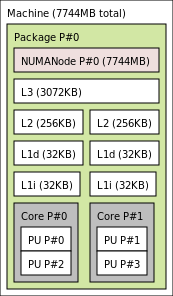
\includegraphics[width=0.25\textwidth]{Figures/ideapad-topo.png}
	\linebreak
	\caption{Η τοπολογία ενός Intel\textsuperscript{\textregistered} Core\textsuperscript{\texttrademark} i3-7100U.}
	\label{fig:ideapad-topo}
\end{figure}


\section{Συστήματα NUMA}
\label{sec:NUMA Systems}
Στην Υποενότητα \ref{ssec:Classification based on memory organization} περιγράφηκε η οργάνωση των συστημάτων ανομοιόμορφης προσπέλασης μνήμης (NUMA), τα οποία αποτελούν αρχιτεκτονική εξέλιξη των Συμμετρικών Πολυεπεξεργαστών (SMPs) που επιτρέπει την κατασκευή μεγαλύτερων παράλληλων συστημάτων.

Η πιο συχνή υλοποίηση των συστημάτων NUMA είναι ως ένα σύνολο κόμβων τύπου SMP που διαθέτουν ιεραρχία κρυφών μνημών συνδεδεμένους μεταξύ τους με ένα δίκτυο διασύνδεσης \cite{dobson2003linux}. Το δίκτυο διασύνδεσης μπορεί να είναι δακτύλιος (ring), διακοπτικό δίκτυο τύπου crossbar, από σημείο σε σημείο (point-to-point) ή πλέγμα (mesh).

Η εξασφάλιση της συνοχής των κρυφών μνημών συνήθως επιτυγχάνεται με τη χρήση ενός πρωτοκόλλου εντός του κόμβου και ενός δεύτερου πρωτοκόλλου μεταξύ των κόμβων. Όπως αναφέρθηκε νωρίτερα, ένας κόμβος SMP βασίζεται σε δίαυλο, ενώ η επικοινωνία μεταξύ των κόμβων γίνεται με πιο πολύπλοκα δίκτυα διασύνδεσης. Για το λόγο αυτό, το πρωτόκολλο συνοχής εντός του κόμβου είναι τύπου παρακολούθησης (snooping protocol), ενώ αυτό μεταξύ των κόμβων βασίζεται σε καταλόγους (directory-based protocol). Φυσικά, σε διαφορετικές οργανώσεις συστημάτων NUMA μπορούμε να συναντήσουμε και άλλες στρατηγικές επίτευξης συνοχής, όπως αυτή της μη αποθήκευσης κοινόχρηστων δεδομένων στις κρυφές μνήμες.

Όπως γίνεται γρήγορα αντιληπτό, ο προγραμματισμός αυτών των συστημάτων συνήθως απαιτεί να εστιάσουμε στην τοπικότητα, δηλαδή τη χρήση πόρων που βρίσκονται στη μικρότερη δυνατή απόσταση και την μείωση της επικοινωνίας μεταξύ των κόμβων \cite{bligh2004linux}. Για την επίτευξη της τοπικότητας και άρα τη συγγραφή πιο αποδοτικών προγραμμάτων, η εκμετάλλευση πληροφορίας που σχετίζεται με την τοπολογία είναι απαραίτητη.

% Ήδη από την έκδοση 2.5 του Linux Kernel προστέθηκε η βασική υποδομή για υποστήριξη συστημάτων NUMA, που περιλαμβάνει μεταξύ άλλων αναγνώριση της τοπολογίας, δέσμευση μνήμης και χρονοδρομολόγηση διεργασιών \cite{dobson2003linux}.

Στο Σχήμα \ref{fig:parade-topo} φαίνεται η οργάνωση του \texttt{parade}, ενός NUMA συστήματος με τέσσερις κόμβους τύπου SMP που διαθέτει η Ομάδα Παράλληλης Επεξεργασίας του Πανεπιστημίου Ιωαννίνων και η οργάνωσή του αποτελεί την πλέον συνηθισμένη.

\begin{figure}[t]
	\centering
	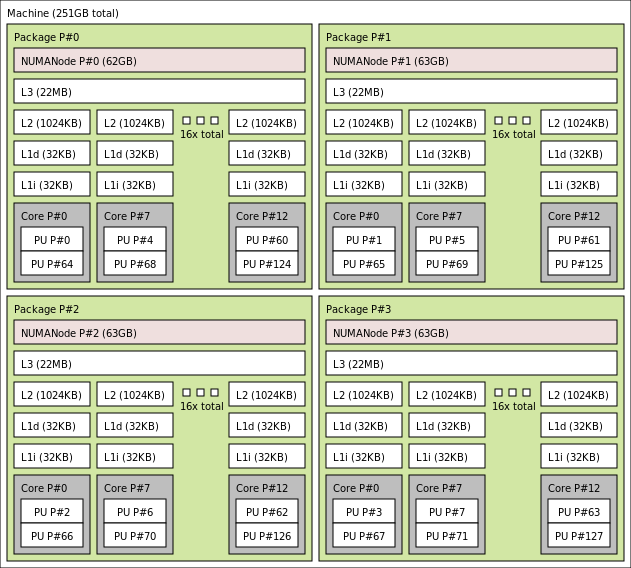
\includegraphics[width=0.8\textwidth]{Figures/parade-topo.png}
	\linebreak
	\caption{Η τοπολογία ενός Dell PowerEdge R840 με 4 Intel\textsuperscript{\textregistered} Xeon\textsuperscript{\textregistered} Gold 6130.}
	\label{fig:parade-topo}
\end{figure}


\section{Βοηθητικά Εργαλεία}
\label{sec:Utility Tools}
Για την εκμετάλλευση της τοπολογίας ενός συστήματος έχουν αναπτυχθεί διάφορα εργαλεία όπως η βιβλιοθήκη Portable Hardware Locality (hwloc) και η \texttt{libnuma}.

\subsection{hwloc}
Η βιβλιοθήκη Portable Hardware Locality παρέχει μία φορητή αφαίρεση (abstraction) της τοπολογίας που διαθέτουν υπολογιστικά συστήματα με σύγχρονες αρχιτεκτονικές. Ο κύριος λόγος χρήσης της είναι η συγκέντρωση πληροφοριών σχετικά με πολύπλοκα παράλληλα συστήματα, με στόχο την κατάλληλη και αποδοτική εκμετάλλευσή τους \cite{broquedis2010hwloc}. 

\noindent Τα λειτουργικά συστήματα που υποστηρίζονται είναι τα εξής:
\begin{itemize}
	\item Linux
	\item Solaris, AIX, HP-UX
	\item NetBSD, FreeBSD, kFreeBSD/GNU
	\item Darwin / OS X
	\item Microsoft Windows
\end{itemize}

\subsubsection{Τα στοιχεία που απαρτίζουν την τοπολογία}
Η hwloc μπορεί να αναγνωρίσει τα εξής στοιχεία υλικού:
\begin{itemize}
	\item Κόμβους συστημάτων NUMA (NUMA nodes)
	\item Υποδοχές επεξεργαστών (packages)
	\item Κρυφές μνήμες (caches)
	\item Πυρήνες (cores)
	\item H/W threads (PUs - Processing Units)
	\item Σύσκευές εισόδου-εξόδου όπως:
	\begin{itemize}
		\item Συσκευές PCI
		\item Επιταχυντές OpenCL, CUDA και Xeon Phi
		\item Προσαρμογείς δικτύου (network interfaces) όπως InfiniBand	
	\end{itemize}
\end{itemize}

Με την ορολογία της hwloc στη διάθεση μας, ας ανατρέξουμε στο Σχήμα \ref{fig:parade-topo} που απεικονίζεται η τοπολογία του συστήματος parade. Στο σχήμα αυτό βλέπουμε 4 επεξεργαστές ο καθένας εκ των οποίων διαθέτει 12 πυρήνες, και ιεραρχία κρυφών μνημών τριών επιπέδων (L1i \& L1d, L2, L3). Τα επίπεδα ένα και δύο των κρυφών μνημών είναι κοινά ανά πυρήνα, ενώ το επίπεδο τρία είναι κοινό για όλους τους πυρήνες του επεξεργαστή. Επίσης, κάθε πυρήνας διαθέτει δύο H/W threads τα οποία μοιράζονται τους πόρους του πυρήνα (π.χ. κρυφές μνήμες).


\subsection{libnuma}



\section{Χρήση τοπολογίας στο OpenMP}
\label{sec:Topology in OpenMP}
Η διπλωματική εργασία περιέχει $\nu$ κεφάλαια.

\chapter{Συγχρονισμός με barriers}
\label{ch:Synchronization with Barriers}
Όπως έχουμε ήδη αναφέρει σε προηγούμενα κεφάλαια, ο προγραμματισμός συστημάτων κοινόχρηστου χώρου διευθύνσεων βασίζεται συνήθως στη χρήση νημάτων, ο συγχρονισμός μεταξύ των οποίων είναι ιδιαίτερα σημαντικός καθώς εξασφαλίζει τη συνέπεια των δεδομένων και την ορθότητα του προγράμματος.

Μία από τις πιο διαδεδομένες μεθόδους συγχρονισμού είναι η \textit{κλήση φραγής}, γνωστή και ως barrier. Όταν στον πηγαίο κώδικα υπάρχει μία κλήση φραγής και συναντηθεί από ένα νήμα, τότε το νήμα περιμένει σε αυτό το σημείο την άφιξη των υπόλοιπων νημάτων, πριν μπορέσουν όλα μαζί να συνεχίσουν την εκτέλεση του κώδικα που ακολουθεί την κλήση φραγής.

%Οι κλήσεις φραγής είναι ιδιαίτερα χρήσιμες για τον διαχωρισμό των φάσεων ενός προγράμματος. Για παράδειγμα, αν θέλουμε να παραλληλοποιήσουμε ένα πρόγραμμα το οποίο υπολογίζει με κάποιο τρόπο τα στοιχεία ενός διδιάστατου πίνακα $A$ (1\textsuperscript{η} φάση) και στη συνέχεια αυτός ο πίνακας χρησιμοποιείται για τον υπολογισμό ενός άλλου πίνακα $B$ (2\textsuperscript{η} φάση), μία κλήση φραγής ανάμεσα στις δύο φάσεις θα εξασφαλίσει ότι πρώτα θα ολοκληρωθεί ο υπολογισμός ολόκληρου του πίνακα $Α$ και μετά θα συνεχίσουν τα νήματα στη δεύτερη φάση. 

Οι κλήσεις φραγής είναι ιδιαίτερα χρήσιμες για τον διαχωρισμό των φάσεων ενός προγράμματος. Για παράδειγμα, αν θέλουμε να παραλληλοποιήσουμε ένα πρόγραμμα το οποίο υλοποιεί μία επαναληπτική μέθοδο (π.χ. conjugate gradient method), θα πρέπει να χρησιμοποιήσουμε κλήση φραγής ανάμεσα στις επαναλήψεις $n$ και $n+1$ ώστε να μην προχωρήσει κάποιο νήμα στην επανάληψη $n+1$ ενώ δεν έχει ολοκληρωθεί ο υπολογισμός της επανάληψης $n$.

%Οι κλήσεις φραγής εκτός από το συγχρονισμόυ νημάτων μπορούν να χρησιμοποιηθούν και για το συγχρονισμό διεργασιών, κάτι που όμως δεν θα μας απασχολήσει στο πλαίσιο της παρούσας διπλωματικής εργασίας.

\section{Υλοποιήσεις barrier}
\label{sec:Barrier Implementations}
Παρόλο που η λογική των κλήσεων φραγής είναι αρκετά απλή, υπάρχει πληθώρα αλγορίθμων για την υλοποίησή τους.

Μία πρώτη κατηγορία κλήσεων φραγής αποτελούν οι κεντρικοποιημένες κλήσεις φραγής (centralized barriers). Κάθε νήμα ενημερώνει μία κοινόχρηστη κατάσταση, ώστε να σημάνει την άφιξη του και έπειτα ελέγχει συνεχώς αυτή την κατάσταση μέχρι να αντιληφθεί ότι έφτασαν όλα τα νήματα. Μόλις φτάσουν όλα τα νήματα, το νήμα συνεχίζει την εκτέλεση του κώδικα που ακολουθεί μετά την κλήση φραγής. Στην πιο απλή της μορφή, η κοινόχρηστη κατάσταση μπορεί να είναι μερικές κοινόχρηστες μεταβλητές που χρησιμοποιούνται για παράδειγμα για τη μέτρηση του πλήθους των νημάτων που αφίχθησαν στον barrier.

Καθώς οι κλήσεις φραγής χρησιμοποιούνται επαναληπτικά, για παράδειγμα όταν υπάρχει ένας barrier στο τέλος ενός βρόγχου \texttt{for}, κατά τη διάρκεια μίας κλήσης τα νήματα θα πρέπει να πραγματοποιήσουν δύο ελέγχους. Έναν έλεγχο που θα εξασφαλίζει ότι όλα τα νήματα έφυγαν από την προηγούμενη κλήση φραγής και έναν έλεγχο που θα εξασφαλίζει ότι όλα τα νήματα έφτασαν στην τρέχουσα κλήση φραγής. Ο έλεγχος για το αν τα νήματα έφυγαν από την προηγούμενη κλήση φραγής είναι απαραίτητος καθώς σε αντίθετη περίπτωση μπορεί να δημιουργηθεί πρόβλημα στο διαχωρισμό δύο διαδοχικών κλήσεων φραγής από κάποιο υποσύνολο των νημάτων. Πιο συγκεκριμένα, όταν υπάρχει μία κοινόχρηστη κατάσταση, υπάρχει η πιθανότητα ένα ή περισσότερα νήματα να εγκλωβιστούν στην προηγούμενη κλήση φραγής, την ώρα που κάποια άλλα έχουν μεταβεί στην επόμενη και ως συνέπεια το πρόγραμμα να οδηγηθεί σε αδιέξοδο (deadlock).

Η λύση για την αποφυγή του διπλού ελέγχου με ταυτόχρονη αποφυγή αδιεξόδου, είναι η εισαγωγή της πληροφορίας \texttt{sense} η οποία παίρνει τιμές \texttt{true} (1) ή \texttt{false} (0). Η πληροφορία \texttt{sense} είναι κοινόχρηστη και η τιμή της αντιστρέφεται μεταξύ δύο διαδοχικών χρήσεων του barrier. Λόγω αυτής της αντιστροφής, η τιμή \texttt{sense} χρησιμοποιείται για το διαχωρισμό μεταξύ διαδοχικών χρήσεων ενός barrier. Η τεχνική αυτή είναι γνωστή ως \textit{sense reversal}, ενώ οι κλήσεις φραγής που τη χρησιμοποιούν είναι γνωστές ως \textit{sense reversing barriers}.

Το μειονέκτημα των κεντρικοποιημένων κλήσεων φραγής είναι οι συνεχόμενες προσβάσεις από όλα τα νήματα σε μία μόνο κοινόχρηστη τοποθεσία. Το πρόβλημα αυτό οδήγησε στην πρόταση υλοποιήσεων που χρησιμοποιούν μεθόδους οπισθοδρόμησης (backoff) όπου ουσιαστικά οι προσβάσεις γίνονται με μεγαλύτερα χρονικά διαστήματα μεταξύ τους. Παράδειγμα μιας τέτοιας μεθόδου αποτελεί η μέθοδος εκθετικής οπισθοδρόμησης (exponential backoff). Αν και με τη χρήση οπισθοδρόμησης παρατηρήθηκε ουσιαστική μείωση της κίνησης στο δίκτυο διασύνδεσης\footnote{Παρατηρήθηκε ταυτόχρονη αύξηση της καθυστέρησης του barrier, δηλαδή του χρόνου μεταξύ της τελευταίας άφιξης και της τελευταίας αναχώρησης από τον barrier.}, δεν επιτυγχάνεται ικανοποιητική κλιμακωσιμότητα των κεντρικοποιημένων κλήσεων φραγής σε μεγάλα συστήματα κάποιων εκατοντάδων επεξεργαστών \cite{mellor1991algorithms}.

Τις συνθήκες υψηλού ανταγωνισμού που υπάρχουν στις κεντρικοποιημένες κλήσεις φραγής μπόρεσε να αντιμετωπίσει ο \textit{combining tree barrier}. Η ιδέα πίσω από αυτή την υλοποίηση είναι η ύπαρξη πολλών μικρών barriers που αποτελούν τους κόμβους-φύλλα μιας δεντρικής δομής δεδομένων και στους οποίους ανατίθενται γνήσια υποσύνολα νημάτων. Κάθε κόμβος τοποθετείται σε διαφορετικά τμήματα μνήμης (memory modules), έτσι ώστε οι προσβάσεις στη μνήμη να μοιράζονται μεταξύ των κόμβων και να μην εστιάζονται σε μία μόνο τοποθεσία όπως συμβαίνει με τους κεντρικοποιημένους barriers. Το τελευταίο νήμα που θα φτάσει σε κάθε barrier-φύλλο (leaf barrier) συνεχίζει διαδίδοντας ενημερώσεις προς τη ρίζα του δέντρου. Όταν κάποιο νήμα καταφέρει να φτάσει στη ρίζα του δέντρου, αυτό σημαίνει ότι όλα τα νήματα που συμμετέχουν στον παράλληλο υπολογισμό έχουν φτάσει στον barrier και η διαδικασία απελευθέρωσής τους από αυτόν μπορεί να ξεκινήσει. Κατά τη διαδικασία απελευθέρωσης, το νήμα που έφτασε στη ρίζα του δέντρου ξεκινά να διαδίδει ενημερώσεις προς τα φύλλα ώστε να επιτραπεί στα νήματα που περιμένουν να συνεχίσουν την εκτέλεση τους.

Ένας παρόμοιος αλγόριθμος με αυτόν του combining tree barrier στον οποίο χρησιμοποιείται δεντρική δομή που έχει τη μορφή δυαδικού δέντρου αποτελεί ο \textit{tournament barrier}. Ο συγχρονισμός μεταξύ των νημάτων πραγματοποιείται μεταξύ δύο νημάτων τη φορά, ενώ το νήμα-εκπρόσωπος που συνεχίζει στο ανώτερο επίπεδο καθορίζεται στατικά και όχι βάσει της σειράς άφιξης, αποφεύγοντας με αυτό τον τρόπο τη χρήση ατομικών εντολών που υλοποιούνται στο υλικό (π.χ. \texttt{fetch\_and\_add()}) και χρησιμοποιούνται από τον combining tree barrier.

Οι παραλλαγές των αλγορίθμων κλήσεων φραγής είναι πάρα πολλές και διαφέρουν άλλες περισσότερο και άλλες λιγότερο μεταξύ τους, ανάλογα με τους στόχους που θέλουν να επιτύχουν αυτοί που τους επινόησαν. Για παράδειγμα, κάποιος μπορεί να προτιμά τη χρήση ή μη ατομικών εντολών που υλοποιούνται στο υλικό (\texttt{fetch\_and\_add()}, \texttt{compare\_and\_swap()} κλπ), τον στατικό ή μη ορισμό των διευθύνσεων μνήμης των κόμβων ενός combining tree barrier, τη χρήση ή μη κλειδαριών (locks) κόκ. Οι διάφορες παραλλαγές στοχεύουν στην επίλυση ζητημάτων που σχετίζονται για παράδειγμα με τις παράλληλες εφαρμογές ή την οργάνωση των υποκείμενων συστημάτων και μπορεί να αφορούν μεταξύ άλλων το πλήθος τον απομακρυσμένων προσβάσεων μνήμης σε συστήματα NUMA, την πολυπλοκότητα χώρου που χρειάζεται ο barrier (π.χ. $O(1)$ για χρήση σταθερού πλήθους κοινόχρηστων μεταβλητών ή $O(N)$ όπου $N$ το πλήθος των νημάτων για χρήση πινάκων με κάθε στοιχείο να αντιστοιχεί σε ένα νήμα) ή το ποσό της κίνησης που δημιουργείται στο δίκτυο διασύνδεσης λόγω των πρωτοκόλλων συνοχής κρυφής μνήμης ανάλογα το είδος αυτών.

\section{Barriers στο OpenMP}
\label{sec:Barriers in OpenMP}
Στη διεπαφή προγραμματισμού εφαρμογών OpenMP που περιγράφηκε στο Κεφάλαιο \ref{ch:OpenMP API}, είδαμε ότι οι κλήσεις φραγής χρησιμοποιούνται ευρέως, τόσο έμμεσα (implicit barrier) στο τέλος παράλληλων περιοχών και των περιοχών διαμοιρασμού εργασίας, όσο και άμμεσα (explicit barrier) μέσω της οδηγίας \texttt{barrier}. Συνεπώς, το πόσο αποδοτική ή όχι είναι η υλοποίηση του barrier μπορεί να έχει σημαντικό αντίκτυπο στην συνολική επίδοση της παράλληλης εφαρμογής. % maybe move to next section

Ενδιαφέρον αποτελεί το γεγονός ότι ο ρόλος των κλήσεων φραγής στα πλαίσια του OpenMP είναι διευρυμένος σε σχέση με τις κλήσεις φραγής που περιγράψαμε μέχρι στιγμής. Αυτό συμβαίνει καθώς ο ρόλος τους εκτός από την επίτευξη συγχρονισμού μεταξύ των νημάτων, περιλαμβάνει και την εξασφάλιση ολοκλήρωσης των εργασιών OpenMP (Υποενότητα \ref{ssec:task directive}), των λεγόμενων και OpenMP tasks ή απλώς tasks, τα οποία δημιουργήθηκαν από την παράλληλη ομάδα. Ένα άλλο χαρακτηριστικό του OpenMP είναι το \textit{cancellation}, δηλαδή η δυνατότητα ακύρωσης της εκτέλεσης μιας περιοχής OpenMP, όπως για παράδειγμα μια παράλληλη περιοχή και η μετάβαση των νημάτων στο τέλος αυτής. Σε περίπτωση που ζητηθεί η ακύρωση της εκτέλεσης μιας παράλληλης περιοχής, τα νήματα επιτρέπεται να μεταβούν στο τέλος της ακόμα και αν δεν έχουν προλάβει να αφιχθούν στην έμμεση κλήση φραγής που βρίσκεται αμέσως πριν αυτό. Οπότε, θα πρέπει οι κλήσεις φραγής που χρησιμοποιούνται στα πλαίσια του OpenMP να υποστηρίζουν την ακύρωση ενός barrier και να επιτρέπουν σε νήματα που έχουν ήδη αφιχθεί να φύγουν από τη διαδικασία αναμονής και να συνεχίσουν την εκτέλεσή τους.

Συνεπώς, οι προϋπάρχοντες αλγόριθμοι κλήσεων φραγής που στοχεύουν μόνο στο συγχρονισμό των νημάτων, είτε θα πρέπει να προσαρμοστούν κατάλληλα για την εξασφάλιση της ολοκλήρωσης των tasks και την υποστήριξη του cancellation, είτε θα πρέπει να επαναδιατυπωθούν από την αρχή για λόγους καλύτερης σχεδίασης, που εν τέλει μπορεί να επηρεάσει την απλότητα και την απόδοση της υλοποίησης.

\section{Ο barrier του OMPi}
\label{sec:OMPi's barrier}
Ο αλγόριθμος του barrier που χρησιμοποιείται στο μεταφραστή OMPi έχει προκύψει μετά από πλήθος βελτιώσεων και επανασχεδιάσεων.

Στην πράξη, ο OMPi διαθέτει τρεις διαφορετικούς αλγορίθμους barrier, καθένας από τους οποίους έχει δύο εκδόσεις. Οι εκδόσεις αυτές χρησιμοποιούνται όταν το cancellation είναι ενεργοποιημένο ή όχι. Για λόγους απλότητας και για ευκολότερη κατανόηση των αλγορίθμων, στα πλαίσια αυτής της διπλωματικής εργασίας θα ασχοληθούμε μόνο με τις εκδόσεις που δεν υποστηρίζουν το cancellation. Επιπλέον, για τους ίδιους λόγους θα παραλειφθούν κάποιες λεπτομέρειες υλοποίησης. Οι τρεις διαφορετικοί τύποι barrier είναι οι εξής:
\begin{itemize}
	\item Parallel Barrier (PB): Χρησιμοποιείται στο τέλος παράλληλων περιοχών και εξασφαλίζει τόσο την ολοκλήρωση της εκτέλεσης των tasks, όσο και το συγχρονισμό των νημάτων.
	\item Default Barrier (DB): Είναι η πιο απλή μορφή barrier που χρησιμοποιείται εντός των παράλληλων περιοχών και εξασφαλίζει μόνο το συγχρονισμό των νημάτων καθώς υποθέτει ότι δεν υπάρχουν tasks. Σε περίπτωση που δημιουργηθούν tasks, τα νήματα μεταβαίνουν σε μια πιο πολύπλοκη μορφή barrier, τον task barrier. 
	\item Task Barrier (TB): Στον barrier αυτό μεταβαίνουν τα νήματα αφού ησέλθουν πρώτα στον default barrier με την προϋπόθεση ότι δημιουργήθηκαν tasks. Εξασφαλίζει τόσο την ολοκλήρωση των tasks, όσο και τον συγχρονισμό των νημάτων.
\end{itemize}

Όλα τα δεδομένα του barrier αποθηκεύονται σε μία μεταβλητή τύπου \texttt{struct} που ονομάζεται \texttt{ort\_defbar\_t} και οι συναρτήσεις διαχείρισης και χρήσης του barrier είναι οι ακόλουθες:

\begin{itemize}
	\item \texttt{ort\_default\_barrier\_init()}: Αρχικοποιεί τον barrier.
	\item \texttt{ort\_default\_barrier\_wait()}: Χρησιμοποιείται από τα νήματα για να συγχρονιστούν στον barrier.
	\item \texttt{ort\_default\_barrier\_destroy()}: Καταστρέφει τον barrier.
\end{itemize}

Η ορολογία \textit{default barrier} που χρησιμοποιείται στις παραπάνω συναρτήσεις αφορά τη χρήση του barrier που παρέχεται από τον OMPi και όχι του barrier που πιθανώς παρέχεται από κάποιο EELIB. Γι' αυτό το λόγο δεν θα πρέπει να συγχέεται με τον ένα από τους τρεις τύπους barrier που παρέχει ο OMPi.

Στη δομή ελέγχου EECB του κάθε νήματος υπάρχει ένας barrier ο οποίος όταν το νήμα δημιουργήσει μια παράλληλη περιοχή, δηλαδή γίνει νήμα-αρχηγός, θα χρησιμοποιηθεί για το συγχρονισμό των νημάτων που συμμετέχουν στην ομάδα. Η αρχικοποίηση του barrier γίνεται στη συνάρτηση \texttt{prepare\_master()} η οποία χρησιμοποιείται για την προετοιμασία του νήματος-αρχηγού για την επικείμενη παράλληλη περιοχή (π.χ. καθορισμός μεγέθους ομάδας, ορισμός της εργασίας που θα εκτελετεί).


\subsection{Βασική αρχιτεκτονική}
\label{ssec:Basic barrier architecture}
Η σχεδίαση των barriers του OMPi βασίζεται σε πίνακες ακεραίων σταθερού μεγέθους (\texttt{MAX\_BAR\_THREADS}\footnote{Τρέχουσα τιμή ίση με 256.}). Κάθε στοιχείο αντιστοιχεί σε ένα μόνο νήμα ώστε να μπορούν να πραγματοποιηθούν προσβάσεις χωρίς τη χρήση κλειδαριών για λόγους αμοιβαίου αποκλεισμού. Με αυτό τον τρόπο, όσο αυξάνεται το πλήθος των νημάτων, ο ανταγωνισμός μεταξύ τους παραμένει ανύπαρκτος. Βέβαια, κάθε πίνακας απαιτεί $O($\texttt{MAX\_BAR\_THREADS}$)$ χώρο, όπου \texttt{MAX\_BAR\_THREADS} το μέγιστο πλήθος των νημάτων που υποστηρίζεται και καθορίζεται κατά το χρόνο μετάφρασης.

Μόλις ένα νήμα φτάσει στον barrier γράφει μία τιμή, έστω 1, στο αντίστοιχο στοιχείο του πίνακα για να σηματοδοτήσει την άφιξή του. Στη συνέχεια, ελέγχει συνεχώς (spins) την τιμή του στοιχείου μέχρι να αλλάξει από 1 σε 0. Αυτό συμβαίνει για όλα τα νήματα, με εξαίρεση το νήμα-αρχηγό (master thread) το οποίο διατρέχει όλες τις θέσεις του πίνακα και ελέγχει αν το αντίστοιχο νήμα έχει φτάσει στον barrier, δηλαδή αν η τιμή του στοιχείου \texttt{arrived[x]} ισούται με 1. Μόλις αντιληφθεί ότι όλα τα νήματα έχουν φτάσει, γράφει σε όλες τις θέσεις του πίνακα την τιμή μηδέν η οποία σηματοδοτεί την απελεθέρωση των νημάτων από τον barrier ώστε να συνεχίσουν την εκτέλεσή τους.

Ο ψευδοκώδικας σε γλώσσα C του αλγορίθμου που περιγράφει τη βασική αρχιτεκτονική του barrier φαίνεται στα Προγράμματα \ref{prg:bsc1} και \ref{prg:bsc2}.

\begin{lstlisting}[label=prg:bsc1, caption=Απλός barrier για όλα τα νήματα πλην του νήματος-αρχηγού.]
arrived[myid] = 1;          /* Mark me as arrived. */
while (arrived[myid] == 1)  /* Spin until released. */
    ;
\end{lstlisting}

\begin{lstlisting}[label=prg:bsc2, caption=Απλός barrier για όλα τα νήματα πλην του νήματος-αρχηγού.]
for every thread (i):
    while (arrived[i] != 1)  /* Wait until thread i arrives */
        ;
        
for every thread (i):
    arrived[i] = 0;  /* Release thread i */
\end{lstlisting}

Ο πίνακας \texttt{arrived} θα πρέπει να έχει αρχικοποιηθεί σε μηδέν κατά την αρχικοποίηση του barrier.


\subsection{Parallel Barrier (PB)}
Ο parallel barrier χρησιμοποιείται αποκλειστικά και μόνο στο τέλος των παράλληλων περιοχών ώστε να εξασφαλίσει τόσο την ολοκλήρωση της εκτέλεσης των tasks, όσο και το συγχρονισμό των νημάτων. Στον barrier αυτό χρησιμοποιούνται δύο πίνακες μεγέθους \texttt{MAX\_BAR\_THREADS} αρχικοποιημένοι στο μηδέν.

Αρχικά, όλα τα νήματα πλην του νήματος-αρχηγού μόλις φτάσουν στον barrier γράφουν την τιμή $2$ στη θέση \texttt{arrived[myid]}, όπου \texttt{myid} το αριθμητικό αναγνωριστικό του εκάστοτε νήματος. Στη συνέχεια περιμένουν μέχρι να αλλάξει η τιμή \texttt{arrived[myid]}, ελέγχοντας παράλληλα για το αν υπάρχουν tasks και σε περίπτωση που υπάρχουν τα εκτελούν. Η διαδικασία ελέγχου για tasks είναι χρονοβόρα καθώς το κάθε νήμα δεν ελέγχει μόνο τη δική του ουρά (queue) για να δει αν υπάρχουν διαθέσιμα tasks προς εκτέλεση, αλλά ελέγχει και τις ουρές όλων των υπόλοιπων νημάτων ώστε να να "κλέψει" ένα task και να το εκτελέσει. Η τεχνική αυτή είναι γνωστή ως \textit{work stealing} και στην περίπτωση των NUMA συστημάτων όπου πραγματοποιούνται απομακρυσμένες προσβάσεις μνήμης, ο χρόνος που απαιτείται για να διεκπεραιωθεί αυξάνεται σημαντικά.

Μόλις φτάσουν όλα τα νήματα στον barrier θα έχει εξασφαλιστεί ο συγχρονισμός, οπότε στη συνέχεια πρέπει να εξασφαλιστεί ότι όλα τα tasks έχουν ολοκληρωθεί. Αυτό γίνεται μέσω ενός δεύτερου σημείου συγχρονισμού, στο οποίο θα περιμένουν τα νήματα αφού ολοκληρώσουν την εκτέλεση των tasks που πιθανώς ανέλαβαν κατά την αναμονή τους στο πρώτο σημείο συγχρονισμού.

Ο ψευδοκώδικας σε γλώσσα C του αλγορίθμου του parallel barrier φαίνεται στα Προγράμματα \ref{prg:pb1} και \ref{prg:pb2}.

\begin{lstlisting}[label=prg:pb1, caption=Parallel barrier για όλα τα νήματα πλην του νήματος-αρχηγού.]
/* 1st synchronization point */
arrived[myid] = 2;
while (arrived[myid] == 2)
    if (task_exist)
        check_and_execute_tasks();
    
if (task_exist)
    check_and_execute_tasks();
    
/*2nd synchronization point */
released[myid] = 1;
while (released[myid] == 1)
    ;
\end{lstlisting}


\begin{lstlisting}[label=prg:pb2, caption=Parallel barrier για το νήμα-αρχηγό.]
/* 1st synchronization point */
for every thread (i):
    while (arrived[i] != 2)
        if (task_exist)
            check_and_execute_tasks();
        
for every thread (i):
    arrived[i] = 0;
   
/* 2nd synchronization point */
for every thread (i):
    while (released[i] != 1)
        ;
        
for every thread (i):
    released[i] = 0;
\end{lstlisting}


\noindent Είναι σημαντικό να σημειωθούν τα εξής:
\begin{itemize}
	\item Το \texttt{task\_exist} είναι μία μεταβλητή-σημαία (flag) για το αν έχουν φτιαχτεί tasks.
	\item Aνάμεσα στα δύο σημεία συγχρονισμού, υπάρχει ένας ακόμα έλεγχος για tasks. Αυτός ο έλεγχος καλύπτει την περίπτωση στην οποία το τελευταίο νήμα λίγο πριν φτάσει στο πρώτο σημείο συγχρονισμού, έφτιαξε ένα task, το νήμα-αρχηγός είδε ότι όλα τα νήματα έφτασαν στον barrier και ξεκίνησε την απελευθέρωσή τους από το πρώτο σημείο συγχρονισμού, πριν προλάβει κάποιο νήμα να ελέγξει για tasks και να εντοπίσει το νέο task.
	\item Κάθε στοιχείο των πινάκων \texttt{arrived} και \texttt{released} καταλαμβάνει χώρο όσο μία γραμμή\footnote{Cache line ή cache block: Η ποσότητα πληροφορίας που μεταφέρεται μεταξύ κρυφής μνήμης και κύριας μνήμης. Είναι σταθερού μεγέθους και μία τυπική τιμή είναι τα 64 bytes.} της κρυφής μνήμης για την αποφυγή του φαινομένου \textit{false sharing}\footnote{Κατά το φαινόμενο του false sharing, διαφορετικά νήματα ενημερώνουν δεδομένα στην ίδια γραμμή της κρυφής μνήμης, με αποτέλεσμα να δημιουργείται πολύ υψηλή κίνηση στο δίκτυο διασύνδεσης λόγω του πρωτοκόλλου συνοχής κρυφής μνήμης.}. (Ισχύει και για τους τρεις τύπους barrier)
	\item Όσο τα νήματα περιμένουν την απελευθέρωσή τους από το νήμα-αρχηγό, ανά κάποιο σταθερό χρονικό διάστημα, παραχωρούν την προτεραιότητά τους (yield) σε άλλα νήματα ώστε να εκτελεστούν. Το ίδιο συμβαίνει και για το νήμα-αρχηγό όσο περιμένει την άφιξη ενός νήματος στον barrier. (Ισχύει και για τους τρεις τύπους barrier)
\end{itemize}


\subsection{Default Barrier (DB)}
Ο default barrier είναι η πιο απλή μορφή barrier και σε αντίθεση με τον parallel barrier χρησιμοποιείται εντός των παράλληλων περιοχών. Σκοπός του είναι να εξασφαλίσει μόνο το συγχρονισμό των νημάτων καθώς υποθέτει ότι δεν υπάρχουν tasks. Σε περίπτωση όμως που δημιουργηθούν tasks, τα νήματα μεταβαίνουν σε μια πιο πολύπλοκη μορφή barrier, τον task barrier που περιγράφεται στην Υποενότητα \ref{ssec:tb}. 

Ο barrier αυτός είναι σε μεγάλο βαθμό ίδιος με τη βασική αρχιτεκτονική που περιγράφηκε στην Υποενότητα \ref{ssec:Basic barrier architecture}, με τη μόνη διαφορά ότι πραγματοποιεί ελέγχους για την ύπαρξη tasks. Ο έλεγχος για tasks πραγματοποιείται με τον ίδιο τρόπο όπως στον parallel barrier και γι' αυτό δεν θα τον περιγράψουμε περαιτέρω.

Ο ψευδοκώδικας σε γλώσσα C του αλγορίθμου του default barrier φαίνεται στα Προγράμματα \ref{prg:db1} και \ref{prg:db2}.

\begin{lstlisting}[label=prg:db1, caption=Default barrier για όλα τα νήματα πλην του νήματος-αρχηγού.]
arrived[myid] = 1;
while (arrived[myid] == 1)
    if (task_exist)
        goto TB;
\end{lstlisting}

\begin{lstlisting}[label=prg:db2, caption=Default barrier για το νήμα-αρχηγό.]
for every thread (i):
    while (arrived[i] != 2)
        if (task_exist)
            goto TB;

if (task_exist)
    goto TB;
     
for every thread (i):
    arrived[i] = 0;
\end{lstlisting}


\subsection{Task Barrier (TB)}
\label{ssec:tb}
Στον task barrier μεταβαίνουν τα νήματα αφού ησέλθουν πρώτα στον default barrier με την προϋπόθεση ότι δημιουργήθηκαν tasks. Εξασφαλίζει τόσο την ολοκλήρωση των tasks, όσο και τον συγχρονισμό των νημάτων.

Αν και παλιότερα ο parallel barrier ήταν πιο απλός από τον task barrier\footnote{Αποτελούνταν από ένα σημείο συγχρονισμού αντί για δύο.}, στην τρέχουσα μορφή τους είναι σχεδόν ίδιοι. Η μόνη διαφορά τους είναι ότι ο parallel barrier πρώτα ελέγχει αν έχουν φτιαχτεί tasks και στη συνέχεια ψάχνει να βρει στις ουρές όλων των νημάτων κάποιο task για να εκτελέσει. Ο task barrier ξεκινάει αμέσως την αναζήτηση για tasks, μιας και ο έλεγχος της μεταβλητής-σημαίας έχει ήδη γίνει στον default barrier.

Ο ψευδοκώδικας σε γλώσσα C του αλγορίθμου του task barrier φαίνεται στα Προγράμματα \ref{prg:tb1} και \ref{prg:tb2}.

\begin{lstlisting}[label=prg:tb1, caption=Task barrier για όλα τα νήματα πλην του νήματος-αρχηγού.]
/* 1st synchronization point */
arrived[myid] = 2;
while (arrived[myid] == 2)
    check_and_execute_tasks();
    
check_and_execute_tasks();
    
/*2nd synchronization point */
released[myid] = 1;
while (released[myid] == 1)
    ;
\end{lstlisting}

\begin{lstlisting}[label=prg:tb2, caption=Task barrier για το νήμα-αρχηγό.]
/* 1st synchronization point */
for every thread (i):
    while (arrived[i] != 2)
        check_and_execute_tasks();
        
for every thread (i):
    arrived[i] = 0;
   
/* 2nd synchronization point */
for every thread (i):
    while (released[i] != 1)
        ;
        
for every thread (i):
    released[i] = 0;
\end{lstlisting}


\subsection{Απαιτήσεις μνήμης}
\label{ssec:Memory requirements of OMPi's barrier}
Στο \texttt{struct} \texttt{ort\_defbar\_t} που αποθηκεύονται όλα τα δεδομένα του barrier, υπάρχουν τρεις πίνακες. Οι πίνακες αυτοί είναι οι \texttt{arrived} και \texttt{released} που είδαμε να χρησιμοποιούνται στους τρεις τύπους barrier που αναφέραμε νωρίτερα, καθώς και ο πίνακας \texttt{phase} ο οποίος χρησιμοποιείται για την υλοποίηση της τεχνικής sense reversal που περιγράφηκε στην Ενότητα \ref{sec:Barrier Implementations}. Για λόγους διατήρησης της απλότητας των αλγορίθμων η περιγραφή της τεχνικής αυτής παραλείφθηκε.

Κάθε πίνακας αποτελείται από \texttt{MAX\_BAR\_THREADS} (256) στοιχεία, με κάθε στοιχείο να απαιτεί μέγεθος όσο μία γραμμή της κρυφής μνήμης (128 bytes για αρχιτεκτονική \textit{x86-64} ή για επεξεργαστές που είναι άγνωστη η αρχιτεκτονική τους). Άρα, κάθε πίνακας απαιτεί $256 \times 128 \mbox{B} = 32 \mbox{KiB}$ και συνολικά και οι τρεις πίνακες καταλαμβάνουν $96 \mbox{KiB}$ ή αλλιώς $24$ pages\footnote{Σελίδες εικονικής μνήμης. Mέγεθος στον Linux Kernel: 4096 bytes.}.

Επειδή κάθε νήμα διαθέτει barrier, σε ένα σύστημα NUMA στο οποίο δημιουργείται μία παράλληλη ομάδα με 128 νήματα, μόνο οι barriers απαιτούν $128 \times 96 \mbox{KiB} = 12 \mbox{MiB} = 3073$ pages. Σε ένα μικρό σύστημα τύπου SMP, στο οποίο δημιουργούνται 4 νήματα, οι barriers απαιτούν $4 \times 96 \mbox{KiB} = 96$ pages.

Αν στα παραπάνω συνυπολογιστεί ότι υπάρχει υποστήριξη για πολλαπλές ομάδες και εμφωλευμένο παραλληλισμό, γίνεται εύκολα αντιληπτό ότι οι απαιτήσεις σε μνήμη είναι πραγματικά τεράστιες και πιθανότατα οδηγούν και σε μειωμένες επιδόσεις.

\section{Βελτιστοποίηση απαιτήσεων μνήμης του barrier του OMPi}
Στα πλαίσια αυτής της διπλωματικής εργασίας, έγινε προσπάθεια βελτίωσης του barrier σε συστήματα NUMA. Πριν επικεντρωθούμε στις ιδιαιτερότητες των συστημάτων NUMA, προχωρήσαμε σε κάποιες βελτιώσεις που αφορούν τη μείωση των απαιτήσεων μνήμης ανεξαρτήτως του υποκείμενου συστήματος.

Όπως αναφέρθηκε στην Υποενότητα \ref{ssec:Memory requirements of OMPi's barrier}, οι απαιτήσεις μνήμης του OMPi που σχετίζονται με τον barrier είναι ιδιαίτερα αυξημένες. Οι λόγοι που συμβαίνει αυτό είναι οι εξής:
\begin{itemize}
	\item Ένα τυπικό μέγεθος των γραμμών της κρυφής μνήμης είναι 64 αντί για 128 bytes που χρησιμοποιείται σαν μέγεθος γραμμής από τον OMPi.
	\item Η εκμετάλλευση του διαθέσιμου χώρου μνήμης από τους πίνακες \texttt{arrived}, \texttt{released} και \texttt{phase} δεν είναι η βέλτιστη δυνατή.
	\item Το μέγεθος των πινάκων του barrier είναι σταθερό (\texttt{MAX\_BAR\_THREADS}) και καθορίζεται σε χρόνο μετάφρασης του OMPi. Εκτός αυτού, εμμέσως πλην σαφώς, το μέγιστο πλήθος των νημάτων που συμμετέχουν σε μια παράλληλη ομάδα δεν μπορεί να ξεπεράσει το συγκεκριμένο όριο.
	\item Όλα τα νήματα διαθέτουν μεταβλητή τύπου barrier (\texttt{ort\_defbar\_t}) καθώς αποτελεί πεδίο της δομής ελέχου τους (EECB), ακόμα κι αν δεν γίνουν ποτέ νήματα-αρχηγοί.
\end{itemize}

\noindent Οι βελτιώσεις που έγιναν είναι οι ακόλουθες:
\begin{enumerate}
	\item Το μέγεθος των γραμμών της κρυφής μνήμης από 128 bytes άλλαξε σε 64.
	\item Επειδή κάθε στοιχείο των πινάκων \texttt{arrived}, \texttt{released} και \texttt{phase} πιάνει χώρο όσο μία γραμμή της κρυφής μνήμης, δηλαδή 64 bytes, αλλά χρησιμοποιούνται μόλις τα τέσσερα\footnote{Τυπικό μέγεθος ακεραίου σε συστήματα Linux αρχιτεκτονικής 64-bit.} (4) από αυτά, οι τρεις πίνακες συγχωνεύτηκαν σε έναν. Ο πίνακας αυτός ονομάστηκε \texttt{status}.
	\item Στο EECB του κάθε νήματος αποθηκεύεται δείκτης σε μεταβλητή και όχι μεταβλητή τύπου barrier (\texttt{ort\_defbar\_t}), ενώ η δέσμευση του barrier γίνεται δυναμικά σε χρόνο εκτέλεσης μόνο από τα νήματα-αρχηγούς.
	\item Η δέσμευση του πίνακα \texttt{status} γίνεται δυναμικά ανάλογα το μέγεθος της ομάδας, γεγονός που επιτρέπει πέρα από την εξοικονόμηση μνήμης, την υποστήριξη αυθαίρετου πλήθους νημάτων που συμμετέχουν σε μια παράλληλη ομάδα και όχι το πολύ \texttt{MAX\_BAR\_THREADS} νημάτων.
\end{enumerate}

Σε ένα σύστημα NUMA στο οποίο δημιουργείται μία παράλληλη ομάδα με 128 νήματα οι απαιτήσεις μνήμης σε σελίδες (pages) μετά από κάθε μία από τις παραπάνω βελτιώσεις φαίνονται στον Πίνακα \ref{tab:barrier-mem-optimizations}.

\begin{table}[htbp]
\footnotesize
	\centering
		\begin{tabular}{|c||c|c|c|c|c|}
		\hline
		Α/Α Βελτίωσης & Barriers\footnotemark & Πίνακες/Barrier & Στοιχεία/Πίνακα & Μέγεθος στοιχείου & Σελίδες\footnotemark \\
		\hline \hline
		1 & 128 & 3 & 256 & 64 B & 1536 \\
		\hline
		2 & 128 & 1 & 256 & 64 B & 512 \\
		\hline
		3 & 1 & 1 & 256 & 64 B & 4 \\
		\hline
		4 & 1 & 1 & 128 & 64 B & 2 \\
		\hline
		\end{tabular}
		\caption{Οι απαιτήσεις σε μνήμη του barrier του OMPi μετά από κάθε βελτίωση.}
		\label{tab:barrier-mem-optimizations}
\end{table}
\footnotetext{Συνολικό πλήθος μεταβλητών τύπου barrier (\texttt{ort\_defbar\_t}).}
%\footnotetext{Μέγεθος σε bytes.}
\footnotetext{Συνολικό μέγεθος απαιτήσεων μνήμης σε σελίδες (pages).}

%\begin{itemize}
%	\item 3 πίνακες/barrier * 256 στοιχεία/πίνακα * 64 bytes/στοιχείο * 128 barriers \newline = 6 MiB = 1536 pages
%	\item 1 πίνακα/barrier * 256 στοιχεία/πίνακα * 64 bytes/στοιχείο * 128 barriers \newline = 2 MiB = 512 pages
%	\item 1 πίνακα/barrier * 256 στοιχεία/πίνακα * 64 bytes/στοιχείο * 1 barrier \newline = 16 KiB = 4 pages
%	\item 1 πίνακα/barrier * 128 στοιχεία/πίνακα * 64 bytes/στοιχείο * 1 barrier \newline = 8 KiB = 2 pages
%\end{itemize}

Συνεπώς, ο απαιτούμενος χώρος μνήμης μειώθηκε από τα 12 MiB (3073 pages) στα 8 KiB (2 pages), δηλαδή υπήρξε περίπου μία μείωση της τάξης του $99.93\%$ και η οποία είναι ανεξάρτητη του πλήθους των νημάτων που συμμετέχουν στην παράλληλη ομάδα.


\section{Επανασχεδιασμός του barrier του OMPi για συστήματα NUMA}
Παρόλο που η υλοποίηση του υπάρχοντα barrier του OMPi είναι καλή για σχετικά μικρά συστήματα\footnote{Συστήματα με περίπου το πολύ 32 H/W threads.} τύπου UMA, παρατηρήθηκαν μειωμένες επιδόσεις όσον αφορά μεγαλύτερα συστήματα τύπου NUMA. Όπως ήδη αναφέρθηκε στην Ενότητα \ref{sec:NUMA Systems}, ο αποδοτικός προγραμματισμός των συστημάτων NUMA απαιτεί να εστιάσουμε στην αρχή της τοπικότητας μέσω της εκμετάλλευσης πληροφοριών που σχετίζονται με την τοπολογία του υποκείμενου συστήματος. Για το λόγο αυτό πραγματοποιήθηκε επανασχεδιασμός του αλγορίθμου του barrier που χρησιμοποιείται στον OMPi ώστε να λαμβάνει υπόψιν του την ύπαρξη κόμβων NUMA (ή απλώς κόμβων).

\subsection{Σύντομη περιγραφή}
Πιο συγκεκριμένα, υλοποιήθηκε ένας αλγόριθμος combining tree barrier δύο επιπέδων ο οποίος χρησιμοποιείται σε περίπτωση που τα νήματα μιας παράλληλης ομάδας είναι τοποθετημένα\footnote{Δηλαδή όταν η processor binding policy είναι \texttt{true}, \texttt{close}, \texttt{spread} ή \texttt{master}.} σε δύο ή περισσότερους κόμβους. Σε κάθε κόμβο τοποθετείται ένας barrier-φύλλο (leaf barrier) στον οποίο συγχρονίζονται τα νήματα τα οποία είναι τοποθετημένα στον κόμβο αυτό.

Καθώς ο υπάρχων αλγόριθμος βασίζεται στη χρήση πινάκων, θα πρέπει το κάθε νήμα να αντιστοιχίζεται σε μία μοναδική θέση του πίνακα του barrier. Μέχρι τώρα, η αντιστοίχιση γινόταν βάσει του μοναδικού αναγνωριστικού του κάθε νήματος (EEID - Execution Entity ID) καθώς ο πίνακας ήταν ένας και χρησιμοποιούνταν από όλα τα νήματα. Επειδή όμως στο νέο αλγόριθμο υπάρχουν πολλαπλοί barriers και το πλήθος των νημάτων σε κάθε κόμβο/barrier μπορεί να διαφέρει, θα πρέπει να γίνει αντιστοίχιση του μοναδικού αναγνωριστικού του κάθε νήματος σε ένα τοπικό αναγνωριστικό (LID - Local ID) με ισχύ εντός του κόμβου. Τα τοπικά αναγνωριστικά χρησιμοποιούνται τόσο στους barriers-φύλλα, όσο και στον barrier-ρίζα (root barrier), ενώ οι πιθανές τιμές τους κυμαίνονται στο εύρος $[0,T_n)$. Στην περίπτωση των barrier-φύλλων το $T_n$ αντιστοιχεί στο πλήθος των νημάτων που είναι τοποθετημένα στον κόμβο $n$, ενώ στην περίπτωση του barrier-ρίζα αντιστοιχεί στο πλήθος των κόμβων που χρησιμοποιούνται από την παράλληλη ομάδα.

Υπεύθυνοι για το συγχρονισμό εντός των κόμβων είναι τα νήματα με τοπικό αναγνωριστικό ίσο με μηδέν. Αυτά τα νήματα μπορούν να θεωρηθούν ως νήματα-αρχηγοί στο τοπικό επίπεδο των κόμβων. Αφού επιτευχθεί συγχρονισμός σε επίπεδο κόμβου μέσω του barrier-φύλλου, τα τοπικά νήματα-αρχηγοί συνεχίζουν στο επόμενο επίπεδο μεταβαίνοντας στον barrier-ρίζα ώστε να επιτευχθεί και συγχρονισμός σε επίπεδο συστήματος. Στον barrier-ρίζα υπεύθυνος για το συγχρονισμό είναι το νήμα με μοναδικό αναγνωριστικό (EEID) ίσο με μηδέν. Όταν φτάσουν στον barrier-ρίζα όλα τα νήματα-εκπρόσωποι των κόμβων, έχει επιτευχθεί συγχρονισμός σε επίπεδο συστήματος και ξεκινάει η διαδικασία απελευθέρωσης με κατεύθυνση αντίθετη από αυτή της διαδικασίας άφιξης.

\subsection{Λεπτομέρειες υλοποίησης}
Στα πλαίσια της υλοποίησης χρησιμοποιήθηκε η βιβλιοθήκη \texttt{libnuma} για την ανάκτηση πληροφοριών όπως το πλήθος των διαθέσιμων κόμβων NUMA, την αντιστοίχιση των αριθμητικών αναγνωριστικών των επεξεργαστών στα αριθμητικά αναγνωριστικά των κόμβων στους οποίους υπάγονται, καθώς και τη δέσμευση των μεταβλητών τύπου barrier σε συγκεκριμένους κόμβους με σκοπό την επίτευξη της τοπικότητας.

Αρχικά, κατά την εκκίνηση του συστήματος χρόνου εκτέλεσης του OMPi και υπό την προϋπόθεση ότι η βιβλιοθήκη \texttt{libnuma} είναι διαθέσιμη, πραγματοποείται έλεγχος για την εξακρίβωση των κόμβων στους οποίους επιτρέπεται η δέσμευση μνήμης και για κάθε επεξεργαστή υπολογίζεται και αποθηκεύεται ο κόμβος στον οποίο ανήκει.

Στη συνάρτηση \texttt{prepare\_master()} κατά την οποία προετοιμάζεται το νήμα-αρχηγός για την επικείμενη παράλληλη περιοχή, γίνεται υπολογισμός διάφορων πληροφοριών που θα χρησιμοποιηθούν για την αρχικοποίηση του barrier. Οι πληροφορίες αυτές αφορούν:
\begin{itemize}
	\item Τους κόμβους οι οποίοι θα χρησιμοποιηθούν στην παράλληλη περιοχή που ακολουθεί.
	\item Την ανάθεση τοπικών αναγνωριστικών κάθε νήματος. Ένα τοπικό αναγνωριστικό για τον barrier-φύλλο και ένα για τον barrier-ρίζα.
	\item Το πλήθος των νημάτων που θα τοποθετηθούν σε κάθε κόμβο. 
\end{itemize}

Ο υπολογισμός των κόμβων που θα χρησιμοποιηθούν από μια παράλληλη ομάδα γίνεται με τον ακόλουθο τρόπο. Για κάθε νήμα υπολογίζεται το place στο οποίο θα τοποθετηθεί βάσει του place partition και της processor binding policy που βρίσκεται σε ισχύ στη συγκεκριμένη παράλληλη περιοχή. Στη συνέχεια, χρησιμοποιείται ο πρώτος επεξεργαστής του συγκεκριμένου place για την εύρεση του κόμβου στον οποίο ανήκει.

Ο λόγος που χρησιμοποιείται ο πρώτος επεξεργαστής είναι επειδή θεωρούμε ότι όλοι οι επεξεργαστές ενός place ανήκουν στον ίδιο κόμβο, καθώς στη συνάρτηση \texttt{prepare\_master()} είναι αδύνατο να γνωρίζουμε σε ποιον επεξεργαστή ακριβώς θα τοποθετηθεί το νήμα και συνεπώς ποιος κόμβος θα χρησιμοποιηθεί. Στον OMPi, όταν τα OpenMP places καθορίζονται βάσει αυθαίρετου ονόματος, όλοι οι επεξεργαστές που περιλαμβάνονται σε ένα place ανήκουν στον ίδιο κόμβο. Αν όμως οριστούν μέσω ρητής λίστας από τον χρήστη, υπάρχει η πιθανότητα να δημιουργηθούν places των οποίων οι επεξεργαστές ανήκουν σε διαφορετικούς κόμβους. Σε περίπτωση που το νήμα τοποθετηθεί σε κόμβο διαφορετικό από τον κόμβο του πρώτου επεξεργαστή, ο αλγόριθμος λειτουργεί σωστά με τη μόνη διαφορά ότι θα πραγματοποιούνται απομακρυσμένες προσβάσεις μνήμης για το συγχρονισμό του συγκεκριμένου νήματος.

Αφού υπολογιστούν όλες οι απαραίτητες πληροφορίες που αναφέρθηκαν παραπάνω, πραγματοποιείται έλεγχος για να καθοριστεί αν χρειάζεται η χρήση του combining tree barrier ή απλώς \textit{tree barrier} για συντομία. Αν η επικείμενη παράλληλη ομάδα χρησιμοποιεί δύο ή περισσότερους κόμβους, τότε χρησιμοποιείται ο tree barrier. Σε αντίθετη περίπτωση χρησιμοποιείται ο κλασικός barrier του OMPi που περιγράφηκε στην Ενότητα \ref{sec:OMPi's barrier}.

Η μεταβλητή τύπου δείκτη σε barrier που υπήρχε στη δομή ελέγχου EECB των νημάτων αντικαταστάθηκε με έναν πίνακα δεικτών σε barrier μεγέθους $N+1$, όπου $N$ το πλήθος των διαθέσιμων κόμβων. Οι πρώτοι $N$ δείκτες αντιστοιχούν στους barriers-φύλλα, ενώ ο τελευταίος δείκτης αντιστοιχεί στον barrier-ρίζα. Στη συνάρτηση \texttt{prepare\_master()} δεσμεύεται δυναμικά μνήμη για τον πίνακα δεικτών καθώς και για κάθε barrier, μόνο μία φορά πριν την πρώτη χρήση του. Επίσης, σε κάθε κλήση της αρχικοποιείται ο barrier κάθε κόμβου που πρόκειται να χρησιμοποιηθεί στην παράλληλη περιοχή που ακολουθεί, καθώς και ο barrier-ρίζα.

Στο \texttt{struct} \texttt{ort\_defbar\_t} προστέθηκε το πεδίο \texttt{type} που χρησιμοποιείται για τον καθορισμό του τύπου του barrier και οι πιθανές τιμές είναι:
\begin{itemize}
	\item \texttt{FLAT\_BARRIER}: Για τον κλασικό barrier του OMPi.
	\item \texttt{TREE\_BARRIER\_LOCAL}: Για τους barriers-φύλλα του tree barrier.
	\item \texttt{TREE\_BARRIER\_ROOT}: Για τον barrier-ρίζα του tree barrier.
\end{itemize}

\subsection{Ο αλγόριθμος του νέου barrier}
Κατά την υλοποίηση του combining tree barrier που υλοποιήθηκε στον OMPi, τροποποιήθηκαν οι υπάρχουσες συναρτήσεις. Επειδή οι αλλαγές και στους τρεις τύπους barrier είναι ίδιες λόγω της απόκρυψης των λεπτομερειών υλοποίησης της τεχνικής sense reversal, θα γίνει αναφορά μόνο στον νέο αλγόριθμο ενός τύπου και συγκεκριμένα του default barrier.

Στο νέο αλγόριθμο, ο κώδικας του νήματος-αρχηγού εκτελείται από τα τοπικά νήματα-αρχηγούς. Αφού επιτευχθεί συγχρονισμός σε επίπεδο κόμβου, τα τοπικά νήματα-αρχηγοί μεταβαίνουν στον barrier-ρίζα ώστε να επιτευχθεί και συγχρονισμός σε επίπεδο συστήματος.

Ο ψευδοκώδικας σε γλώσσα C του νέου αλγορίθμου του default barrier φαίνεται στα Προγράμματα \ref{prg:db1-new} και \ref{prg:db2-new}.

\begin{lstlisting}[label=prg:db1-new, caption=Ο νέος default barrier για όλα τα νήματα πλην των τοπικών νημάτων-αρχηγών.]
local_id = (barrier_type == FLAT_BARRIER) ? my_eeid : my_lid;

arrived[local_id] = 1;
while (arrived[local_id] == 1)
    if (task_exist)
        goto TB;
\end{lstlisting}

\newpage

\begin{lstlisting}[label=prg:db2-new, caption=Ο νέος default barrier για τα τοπικά νήματα-αρχηγούς.]
for every thread (i):
    while (arrived[i] != 2)
        if (task_exist)
            goto TB;

if (task_exist)
    goto TB;

/* At this point, inter-node synchronization has been achieved. In case of
 * tree barrier, intra-node synchronization should also take place.
 */
if (barrier_type == TREE_BARRIER_LOCAL)
    goto ROOT_DB;

for every thread (i):
    arrived[i] = 0;
\end{lstlisting}

% Σε αυτό το σημείο χρειάζεται να αναφερθεί ότι ο ψευδοκώδικας στο Πρόγραμμα \ref{prg:db2-new} δεν είναι πλήρης. Επειδή ο default barrier έχει την ιδιαιτερότητα να μεταβαίνει στον task barrier όποτε αυτό είναι απαραίτητο, ...
\chapter{Πειραματική Αξιολόγηση}
\label{ch:Experimental Evaluation}
Οι διάφορες υλοποιήσεις που πραγματοποιήθηκαν στα πλαίσια της τρέχουσας διπλωματικής εργασίας αξιολογήθηκαν πειραματικά με τη χρήση μετροπρογραμμάτων (benchmarks) τόσο για την επιβεβαίωση της ορθότητας της υλοποίησης, όσο και για τη μέτρηση των επιδόσεων που επιτεύχθηκαν.


\section{Περιγραφή Συστημάτων}
\label{sec:Systems Description}
Η εκτέλεση των πειραμάτων έγινε σε υπολογιστικά συστήματα NUMA που εκπροσωπούν τόσο διαδεδομένες, όσο και ενδιαφέρουσες αρχιτεκτονικές οργανώσεις. Τα χαρακτηριστικά των συστημάτων αυτών, τόσο από άποψη υλικού, όσο και από άποψη λογισμικού, φαίνονται στους Πίνακες \ref{tab:exp-systems-hardware} και \ref{tab:exp-systems-software}. Η αρχιτεκτονική των επεξεργαστών όλων των συστημάτων είναι η \textit{x86-64} ενώ το μέγεθος μιας γραμμής της κρυφής μνήμης είναι 64 bytes.

Οι μεταφραστές οι οποίοι χρησιμοποιήθηκαν για τη συγκριτική αξιολόγηση του μεταφραστή OMPi είναι ο \textit{GNU C Compiler} (GCC), ο \textit{Intel C Compiler} (ICC)\footnote{Εγκαταστάθηκε μέσω των oneAPI Toolkits της Intel\textsuperscript{\textregistered}.} και ο \textit{Clang}. Ο πηγαίος κώδικας του OMPi μεταφράστηκε με τον GCC, ενώ τα απαιτούμενα πακέτα λογισμικού είναι διαθέσιμα στο Παράρτημα \ref{app:OMPi's software requirements}.

\begin{table}
	\centering
		\begin{tabular}{|c||c|c|c|c|c|c|}
		\hline
		Hostname & Proc. Mfr. & NUMA nodes & Sockets & Cores & H/W threads & RAM \\
		\hline \hline
		\texttt{parade} & Intel & 4 & 4 & 64 & 128 & 256 GB \\
		\hline
		\texttt{paragon} & AMD  & 4 & 2 & 24 & 24 & 16 GB \\
		\hline
%		\texttt{opti3060} & Intel & 1 & 1 & 4 & 4 & 8 GB \\
%		\hline
%		\texttt{ideapad} & Intel & 1 & 1 & 2 & 4 & 8 GB \\
%		\hline
		\end{tabular}
		\caption{Χαρακτηριστικά υλικού των πειραματικών συστημάτων.}
		\label{tab:exp-systems-hardware}
\end{table}

\begin{table}
	\centering
		\begin{tabular}{|c||c|c|c|c|c|c|c|}
		\hline
		Hostname & OS & GCC & ICC & Clang & hwloc & Linux kernel \\
		\hline \hline
		\texttt{parade} & CentOS 8 & \texttt{8.4.1} & \texttt{2021.3.0} & \texttt{11.0.0} & \texttt{2.2.0} & \texttt{4.18.0} \\
		\hline
		\texttt{paragon} & CentOS 8 & \texttt{8.4.1} & \texttt{2021.3.0} & \texttt{11.0.0} & \texttt{2.2.0} & \texttt{4.18.0} \\
		\hline
%		\texttt{opti3060} & Ubuntu 18.04.3 & \texttt{7.5.0} & \texttt{N/A} & \texttt{N/A} & \texttt{1.11.9} & \texttt{5.0.0} \\
%		\hline
%		\texttt{ideapad} & Mint 20.2 & \texttt{9.3.0} & \texttt{2021.3.0} & \texttt{10.0.0} & \texttt{2.1.0} & \texttt{5.4.0} \\
%		\hline
		\end{tabular}
		\caption{Χαρακτηριστικά λογισμικού των πειραματικών συστημάτων.}
		\label{tab:exp-systems-software}
\end{table}


\subsection{Parade}
Ο Parade είναι ένα σύστημα Dell PowerEdge R840 με τέσσερις κόμβους NUMA. Κάθε κόμβος διαθέτει 64 GBs μνήμης και έναν επεξεργαστή \textit{Intel\textsuperscript{\textregistered} Xeon\textsuperscript{\textregistered} Gold 6130} ο οποίος αποτελείται από 12 πυρήνες και ιεραρχία κρυφών μνημών τριών επιπέδων (L1i \& L1d, L2, L3). Τα επίπεδα ένα και δύο των κρυφών μνημών είναι κοινά ανά πυρήνα, ενώ το επίπεδο τρία είναι κοινό για όλους τους πυρήνες του επεξεργαστή. Επίσης, κάθε πυρήνας περιέχει δύο H/W threads. Η σχηματική αναπαράσταση της τοπολογίας του φαίνεται στο Σχήμα \ref{fig:parade-topo}.

\subsection{Paragon}
Ο Paragon είναι ένα σύστημα με δύο επεξεργαστές \textit{AMD Opteron\textsuperscript{\texttrademark} Processor 6166 HE}, καθένας από τους οποίους περιλαμβάνει δύο κόμβους NUMA. Κάθε κόμβος διαθέτει 6 πυρήνες του ενός H/W thread και ιεραρχία κρυφής μνήμης τριών επιπέδων αντίστοιχη με τους κόμβους του συστήματος Parade που είδαμε προηγουμένως. Η σχηματική αναπαράσταση της τοπολογίας του φαίνεται στο Σχήμα \ref{fig:paragon-topo}.

Ο λόγος που κάθε επεξεργαστής περιλαμβάνει δύο κόμβους είναι επειδή ουσιαστικά αποτελείται από δύο κυκλώματα επεξεργαστών (dies) των έξι πυρήνων το καθένα, τα οποία συνδέονται μεταξύ τους με ένα δίκτυο διασύνδεσης χαμηλής καθυστέρησης και υψηλού εύρους ζώνης που ονομάζεται HyperTransport, με σκοπό να δημιουργηθεί ένα ολοκληρωμένο κύκλωμα επεξεργαστή με 12 πυρήνες \cite{conway2010cache}. Κάθε die μπορεί να επικοινωνήσει απευθείας με τη μνήμη\footnote{Επειδή περιλαμβάνει ελεγκτή μνήμης (memory controller).}, οπότε λόγω της ύπαρξης δικτύου διασύνδεσης μεταξύ των dies, κάθε επεξεργαστής μπορεί να θεωρηθεί ως ένα σύστημα NUMA δύο κόμβων.


\begin{figure}[t]
	\centering
	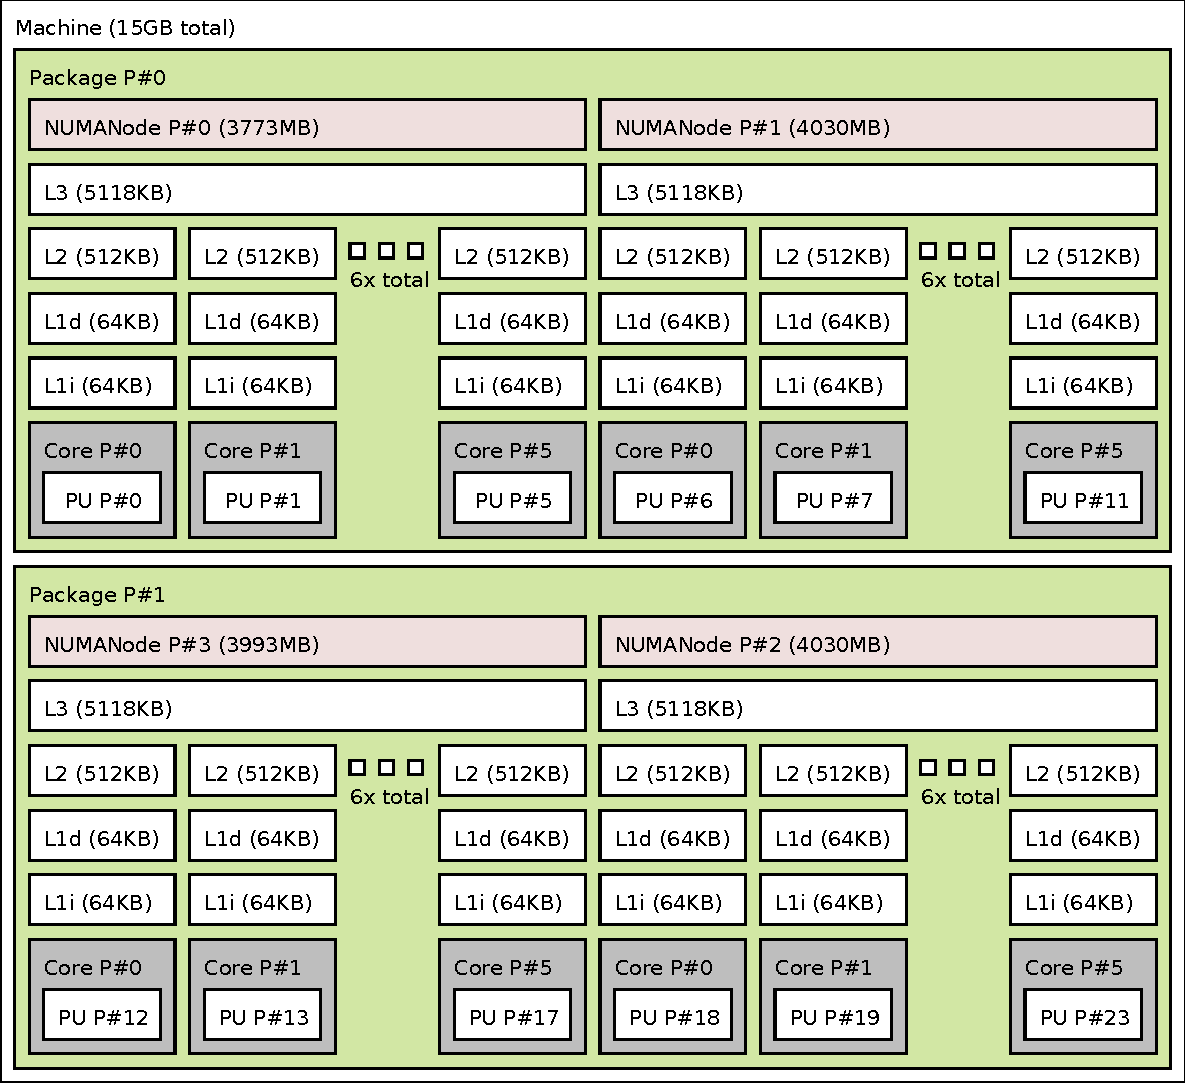
\includegraphics[width=0.8\textwidth]{Figures/paragon-topo.pdf}
	\linebreak
	\caption{Η τοπολογία του συστήματος Paragon.}
	\label{fig:paragon-topo}
\end{figure}


\section{Τοπολογία}
Η υλοποίηση των OpenMP places και OpenMP processor binding policies ελέγχθηκε για την ορθότητά της, δηλαδή  για το αν ικανοποιεί πλήρως τις προδιαγραφές του OpenMP, τόσο με ιδιόχειρα, όσο και με έτοιμα προγράμματα.   Τα έτοιμα προγράμματα ήταν μέρος ενός συνόλου προγραμμάτων ελέγχου ορθότητας τα οποία παρέχονται από τη βιβλιοθήκη \textit{GNU Offloading and Multi Processing Runtime Library} (libgomp) η οποία μεταξύ άλλων, υλοποιεί και τη διεπαφή προγραμματισμού εφαρμογών OpenMP που χρησιμοποιεί ο GCC.


\section{Barrier}
\label{sec:exp-barrier}
Η ορθότητα της υλοποίησης του tree barrier ελέγχθηκε για την ορθότητά της με προγράμματα ελέγχου από τη βιβλιοθήκη libgomp και την \textit{OpenMP Validation Suite V 3.0} \cite{wang2012openmp, ompvalsuite3}. Ο λόγος όμως που αναπτύχθηκε ο tree barrier ήταν οι μειωμένες επιδόσεις του υπάρχοντα barrier του OMPi σε συστήματα NUMA, οπότε αφού εξασφαλίστηκε η ορθότητα της υλοποίησης, εστιάσαμε στο ζήτημα των επιδόσεων με τη χρήση μετροπρογραμμάτων.

\subsection{EPCC OpenMP micro-benchmark suite}
Η \textit{EPCC OpenMP micro-benchmark suite} \cite{bull1999measuring} είναι ένα σύνολο μετροπρογραμμάτων (micro-benchmarks) τα οποία μετράνε το κόστος σε χρόνο (overhead) που απαιτείται για τη διεκπεραίωση λειτουργιών όπως ο συγχρονισμός (π.χ. barrier, κλειδαριές), η \textit{χρονοδρομολόγηση βρόχου} (loop sceduling) και οι πράξεις πινάκων. Η πιο πρόσφατη έκδοση (3.1) υποστηρίζει μέχρι και τις λειτουργίες που προδιαγράφει το OpenMP 3.0.

Τα πειράματα που πραγματοποιήθηκαν επικεντρώθηκαν στη μέτρηση του overhead του barrier, όσο το πλήθος των κόμβων NUMA που χρησιμοποιούνται αυξάνεται. Με αυτό τον τρόπο ελέγχουμε κατά πόσο η εκάστοτε υλοποίηση barrier είναι κλιμακώσιμη. Οι υλοποιήσεις που συγκρίθηκαν είναι αυτές των μεταφραστών OMPi (κλασική και tree barrier), GCC, ICC και Clang. Η OpenMP processor binding policy παρέμεινε σταθερά στην τιμή \texttt{close}, ενώ σε κάθε OpenMP place τοποθετείται μόνο ένα νήμα OpenMP.


\subsubsection{Parade}
Στο Σχήμα \ref{fig:bo-parade-default-places} φαίνεται το overhead του barrier κάθε μεταφραστή όταν χρησιμοποιούνται 1 έως 4 κόμβοι και ένα νήμα ανά core ή H/W thread αντίστοιχα. Αυτό που παρατηρούμε, είναι ότι όταν \texttt{OMP\_PLACES="cores"}, για ένα κόμβο ο OMPi έχει το μικρότερο overhead, το οποίο όμως αυξάνει κατά πολύ για περισσότερους κόμβους. Στην περίπτωση που \texttt{OMP\_PLACES="threads"}, ο OMPi έχει εκθετική αύξηση του overhead για 2 ή περισσότερους κόμβους. Ο tree barrier και στις δύο περιπτώσεις έχει σαφώς καλύτερες επιδόσεις σε σχέση με τον κλασικό barrier του OMPi, ενώ το overhead του αυξάνεται με αρκετά μικρό ρυθμό. Εξαίρεση αποτελεί η περίπτωση που χρησιμοποιείται ένας μόνο κόμβος, κατά την οποία o tree barrier είναι λίγο πιο αργός από τον κλασικό barrier. % Για καλύτερη κατανόηση δείτε το Σχήμα \ref{fig:bo-parade-ompionly}.

%\begin{figure}[t]
%	\centering
%	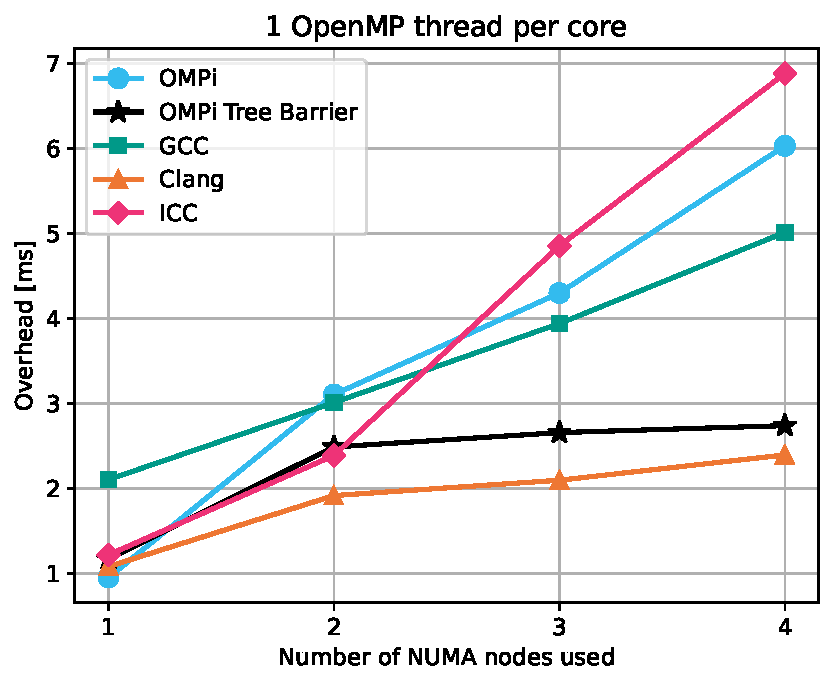
\includegraphics[width=0.7\textwidth]{Figures/epcc_20210823_175412/default-places_cores_close.pdf}
%	\linebreak
%	\caption{Barrier overhead στον Parade: OMP\_PLACES=cores.}
%	\label{fig:bo-parade-cores}
%\end{figure}
%
%\begin{figure}[t]
%	\centering
%	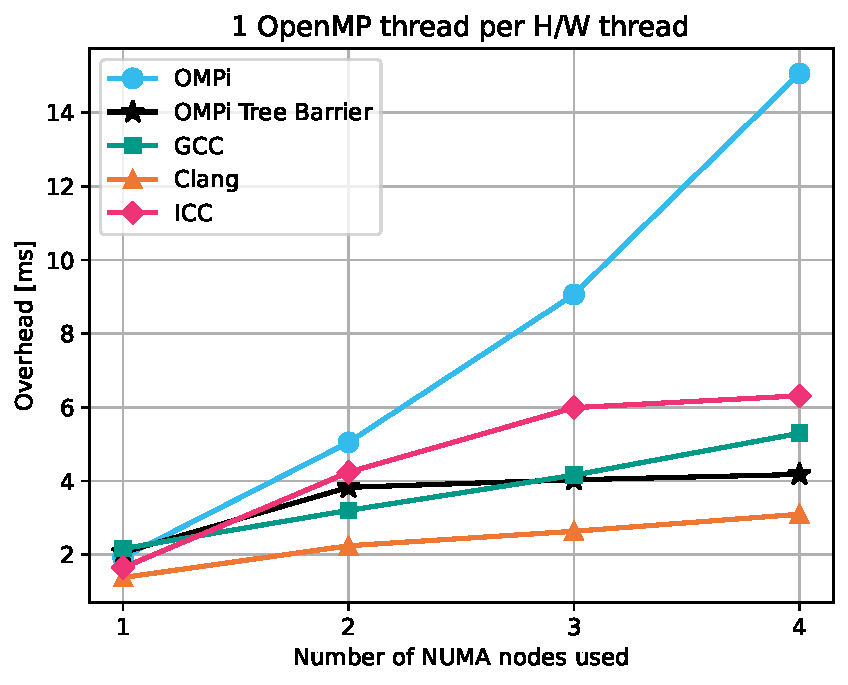
\includegraphics[width=0.7\textwidth]{Figures/epcc_20210823_175412/default-places_threads_close.pdf}
%	\linebreak
%	\caption{Barrier overhead στον Parade: OMP\_PLACES=threads.}
%	\label{fig:bo-parade-threads}
%\end{figure}

\begin{figure}
    \centering
    \begin{minipage}{0.5\textwidth}
        \centering
        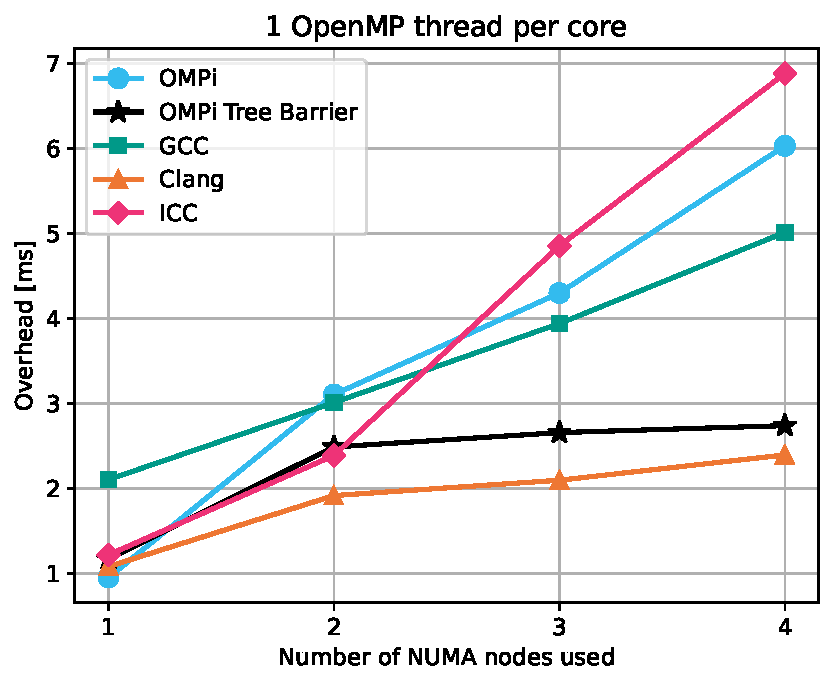
\includegraphics[width=1\textwidth]{Figures/epcc_20210823_175412/default-places_cores_close.pdf}
		\texttt{OMP\_PLACES=cores}
    \end{minipage}\hfill
    \begin{minipage}{0.5\textwidth}
        \centering
        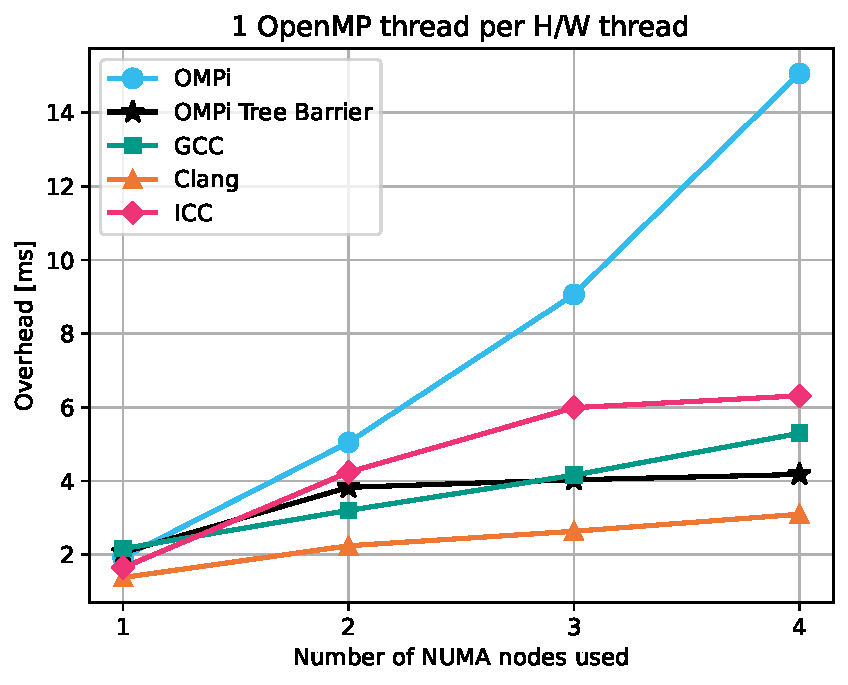
\includegraphics[width=1\textwidth]{Figures/epcc_20210823_175412/default-places_threads_close.pdf}
        \texttt{OMP\_PLACES=threads}
    \end{minipage}
    \caption{Barrier overhead στον Parade (Default places).}
    \label{fig:bo-parade-default-places}
\end{figure}

%\begin{figure}
%    \centering
%    \begin{minipage}{0.5\textwidth}
%        \centering
%        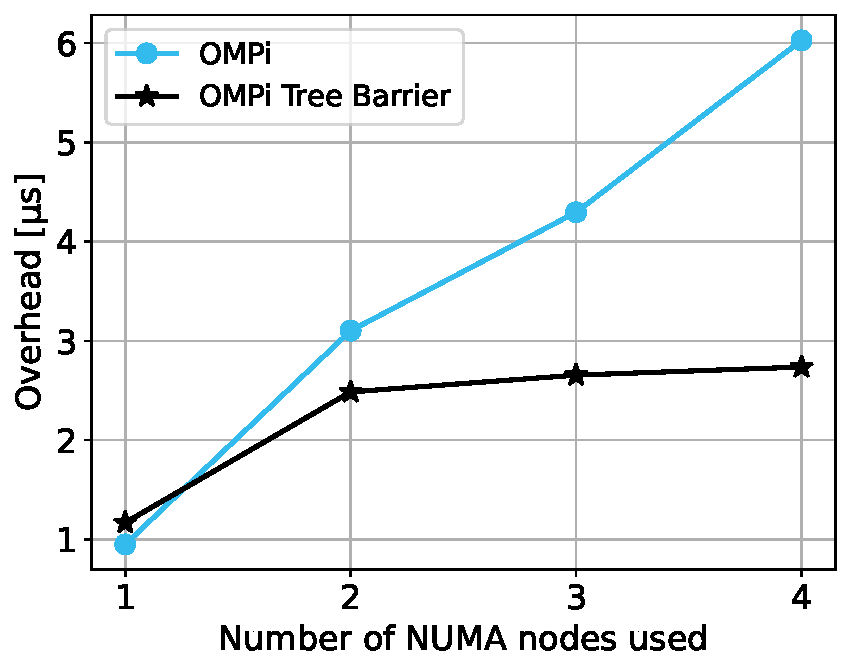
\includegraphics[width=1\textwidth]{Figures/epcc_20210823_175412/ompi_default-places_cores_close.pdf}
%		\texttt{OMP\_PLACES=cores}
%    \end{minipage}\hfill
%    \begin{minipage}{0.5\textwidth}
%        \centering
%        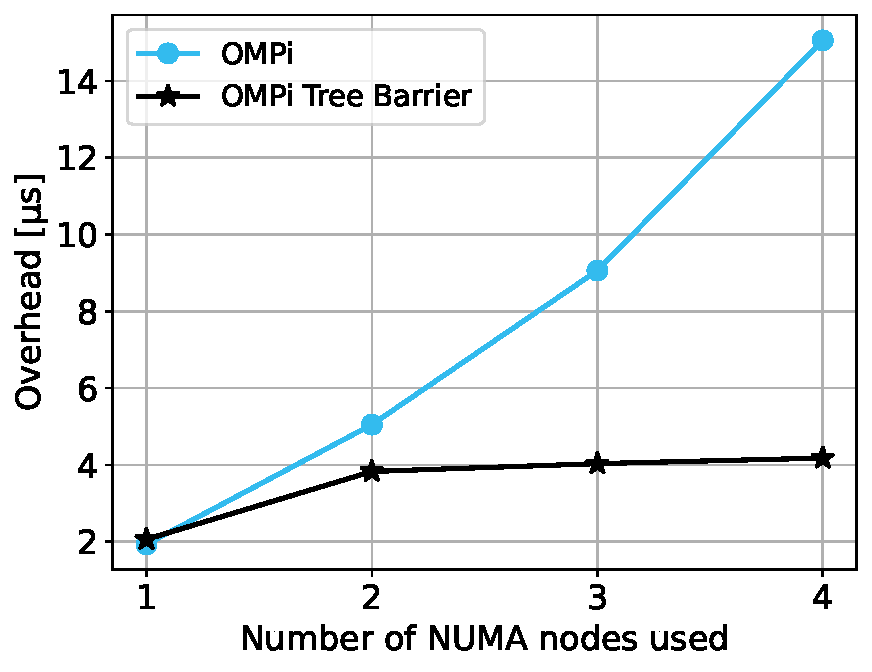
\includegraphics[width=1\textwidth]{Figures/epcc_20210823_175412/ompi_default-places_threads_close.pdf}
%        \texttt{OMP\_PLACES=threads}
%    \end{minipage}
%    \caption{Barrier overhead στον Parade για τους barriers του OMPi (Default places).}
%    \label{fig:bo-parade-ompionly}
%\end{figure}

Η σύγκριση που πραγματοποιήθηκε, ναι μεν είναι σωστή από την πλευρά του χρήστη καθώς χρησιμοποιείται το ίδιο abstract name για τον καθορισμό των places, όμως ο κάθε μεταφραστής μετασχηματίζει με διαφορετικό τρόπο το abstract name σε σύνολα από αναγνωριστικά επεξεργαστών. Για παράδειγμα, όταν \texttt{OMP\_PLACES=cores} o GCC τοποθετεί στο place partition με κυκλικό τρόπο (round-robin) ένα core ανά κόμβο. Συνεπώς, αν ο χρήστης επιλέξει ως processor binding policy την \texttt{close}, νήματα που θα τοποθετηθούν σε γειτονικά places, θα καταλήξουν σε διαφορετικούς κόμβους NUMA.

Λόγω της ουσιαστικής διαφοράς στο place partition που χρησιμοποιεί το σύστημα χρόνου εκτέλεσης του κάθε μεταφραστή, πραγματοποιήσαμε επιπλέον μετρήσεις κατά τις οποίες ορίσαμε την τιμή της μεταβλητής \texttt{OMP\_PLACES} χειροκίνητα, βάσει του πώς δημιουργεί το place partition ο κάθε μεταφραστής. Οι μεταφραστές ICC και Clang ορίζουν με τον ίδιο τρόπο το place partition, οπότε προέκυψαν οι τρεις ακόλουθοι τρόποι ορισμού του:
\begin{itemize}
	\item OMPi places: \texttt{OMP\_PLACES="ompi-cores"} και \texttt{OMP\_PLACES="ompi-threads"}.
	\item GCC places: \texttt{OMP\_PLACES="gcc-cores"} και \texttt{OMP\_PLACES="gcc-threads"}.
	\item Clang/ICC places: \texttt{OMP\_PLACES="clang-cores"} και \texttt{OMP\_PLACES="clang-threads"}.
\end{itemize}

Στα Σχήματα \ref{fig:bo-parade-ompi-places}, \ref{fig:bo-parade-gcc-places} και \ref{fig:bo-parade-clang-places} μπορείτε να δείτε τις μετρήσεις οι οποίες πάρθηκαν με όλους τους μεταφραστές να χρησιμοποιούν το ίδιο place partition. Σε όλες τις περιπτώσεις που χρησιμοποιούνται πολλαπλοί κόμβοι είναι εμφανής η επίτευξη καλύτερης επίδοσης του tree barrier σε σχέση με τον κλασικό barrier του OMPi. Το overhead όταν χρησιμοποιούνται δύο κόμβοι είναι σαφώς πιο αυξημένο σε σχέση με όταν χρησιμοποιείται ένας κόμβος, φαινόμενο πλήρως δικαιολογημένο καθώς στην τελευταία περίπτωση δεν πραγματοποιούνται απομακρυσμένες προσβάσεις μνήμης. Όσο το πλήθος των κόμβων αυξάνεται σε τιμές μεγαλύτερες του δύο, παρατηρούμε ότι η αύξηση του overhead είναι πολύ μικρή. %s Το γεγονός αυτό επιβεβαιώνει την κλιμακωσιμότητα του νέου barrier.

Σε μερικά σχήματα είναι ορατές μη αναμενόμενες συμπεριφορές από τον ICC, όπως για παράδειγμα στο Σχήμα \ref{fig:bo-parade-ompi-places} όπου διακρίνεται ένα πολύ μεγαλύτερο overhead για δύο κόμβους σε σχέση με τους τρεις κόμβους. Αυτό το φαινόμενο παρατηρήθηκε στην τρέχουσα έκδοση του ICC μετά από την πιο πρόσφατη αναβάθμιση που πραγματοποιήθηκε ώστε οι εκδόσεις των πακέτων λογισμικού να ταυτίζονται με αυτές του συστήματος Paragon και άρα να μην οδηγηθούμε σε εσφαλμένα συμπεράσματα λόγω διαφορών ανάμεσα στις εκδόσεις.

\begin{figure}
    \centering
    \begin{minipage}{0.5\textwidth}
        \centering
        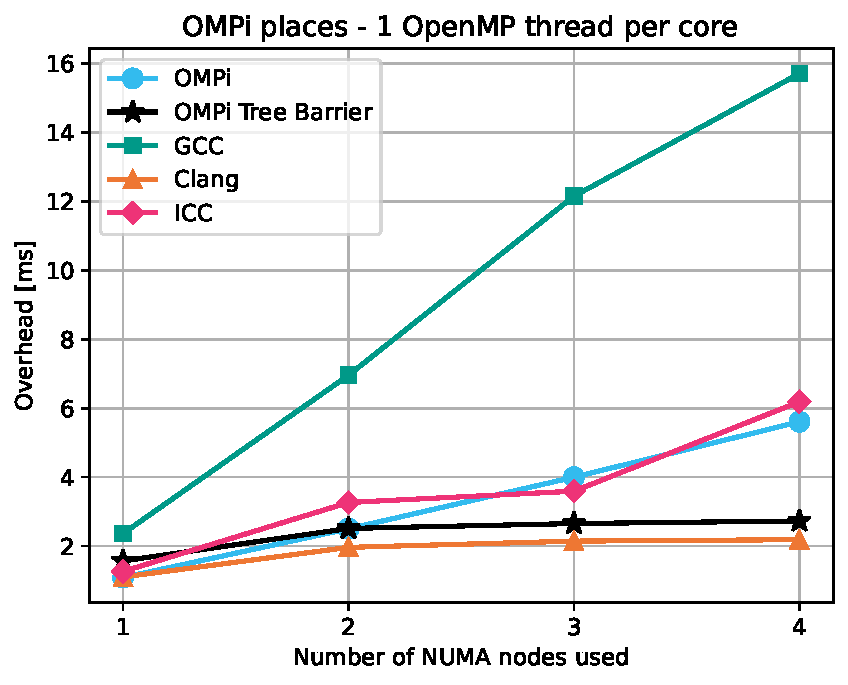
\includegraphics[width=1\textwidth]{Figures/epcc_20210823_175412/ompi-places_cores_close.pdf}
		\texttt{OMP\_PLACES=ompi-cores}
    \end{minipage}\hfill
    \begin{minipage}{0.5\textwidth}
        \centering
        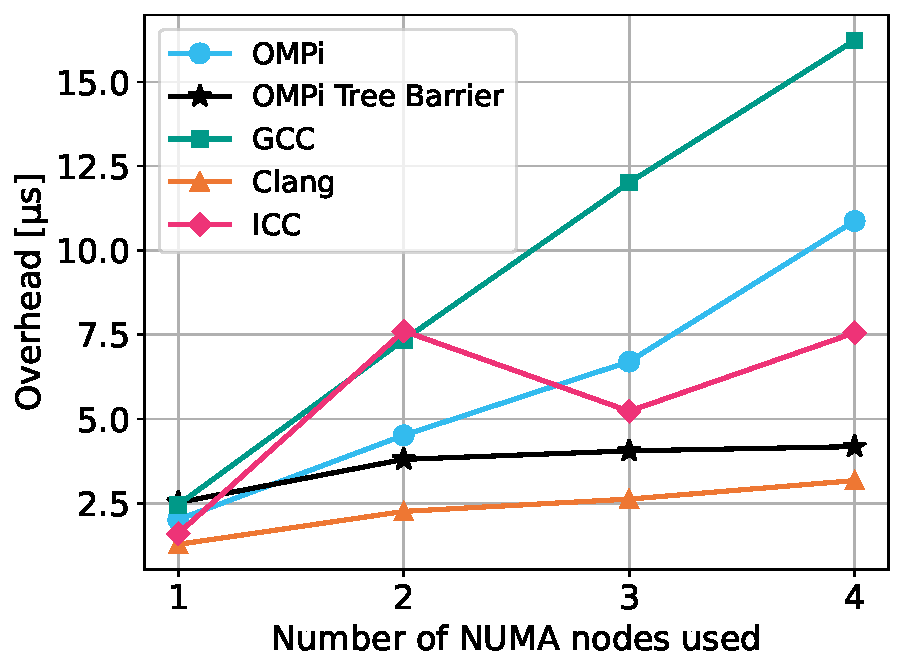
\includegraphics[width=1\textwidth]{Figures/epcc_20210823_175412/ompi-places_threads_close.pdf}
        \texttt{OMP\_PLACES=ompi-threads}
    \end{minipage}
    \caption{Barrier overhead στον Parade (OMPi places).}
    \label{fig:bo-parade-ompi-places}
\end{figure}

\begin{figure}
    \centering
    \begin{minipage}{0.5\textwidth}
        \centering
        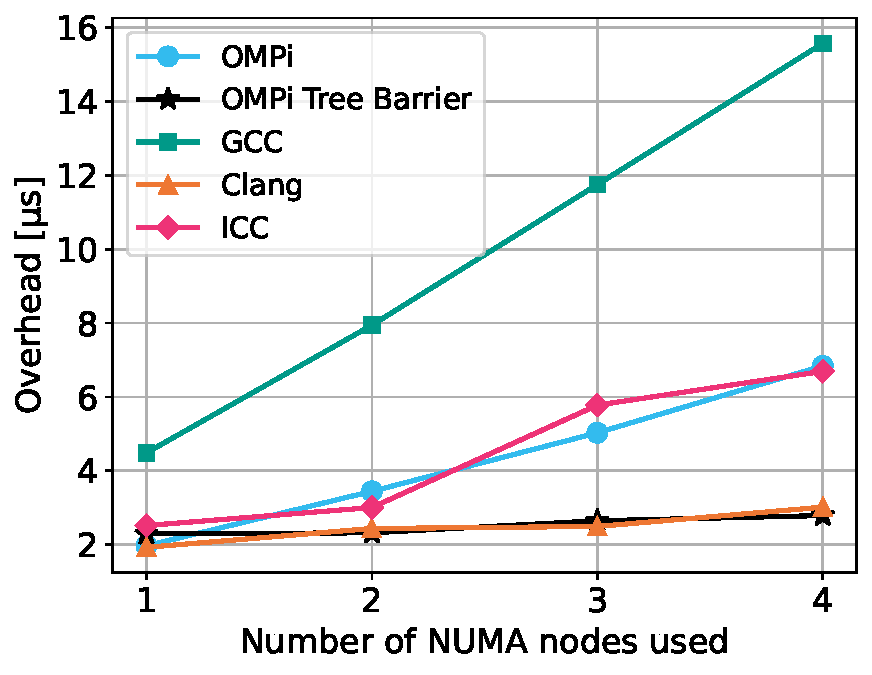
\includegraphics[width=1\textwidth]{Figures/epcc_20210823_175412/gcc-places_cores_close.pdf}
		\texttt{OMP\_PLACES=gcc-cores}
    \end{minipage}\hfill
    \begin{minipage}{0.5\textwidth}
        \centering
        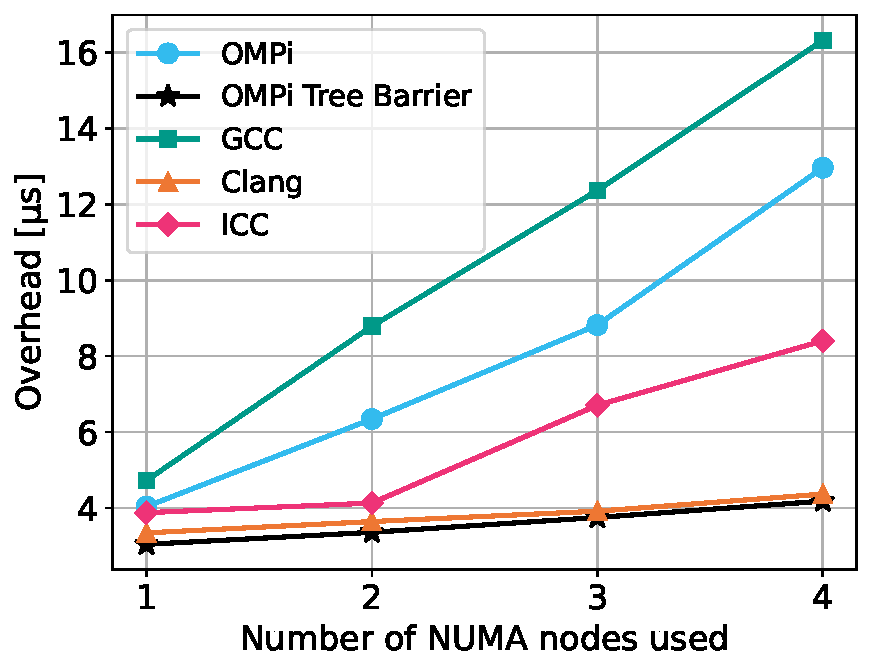
\includegraphics[width=1\textwidth]{Figures/epcc_20210823_175412/gcc-places_threads_close.pdf}
        \texttt{OMP\_PLACES=gcc-threads}
    \end{minipage}
    \caption{Barrier overhead στον Parade (GCC places).}
    \label{fig:bo-parade-gcc-places}
\end{figure}

\begin{figure}
    \centering
    \begin{minipage}{0.5\textwidth}
        \centering
        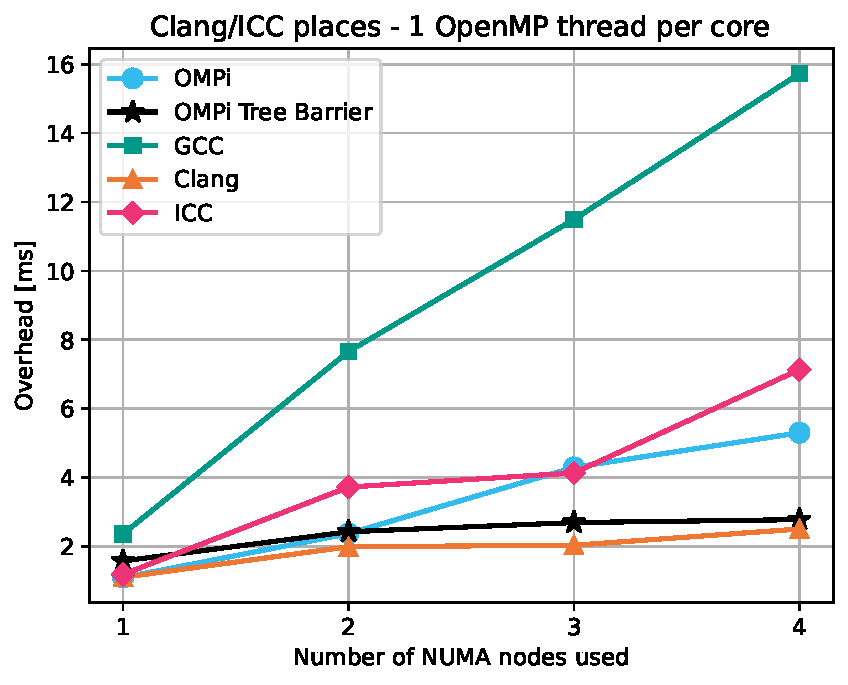
\includegraphics[width=1\textwidth]{Figures/epcc_20210823_175412/clang-places_cores_close.pdf}
		\texttt{OMP\_PLACES=clang-cores}
    \end{minipage}\hfill
    \begin{minipage}{0.5\textwidth}
        \centering
        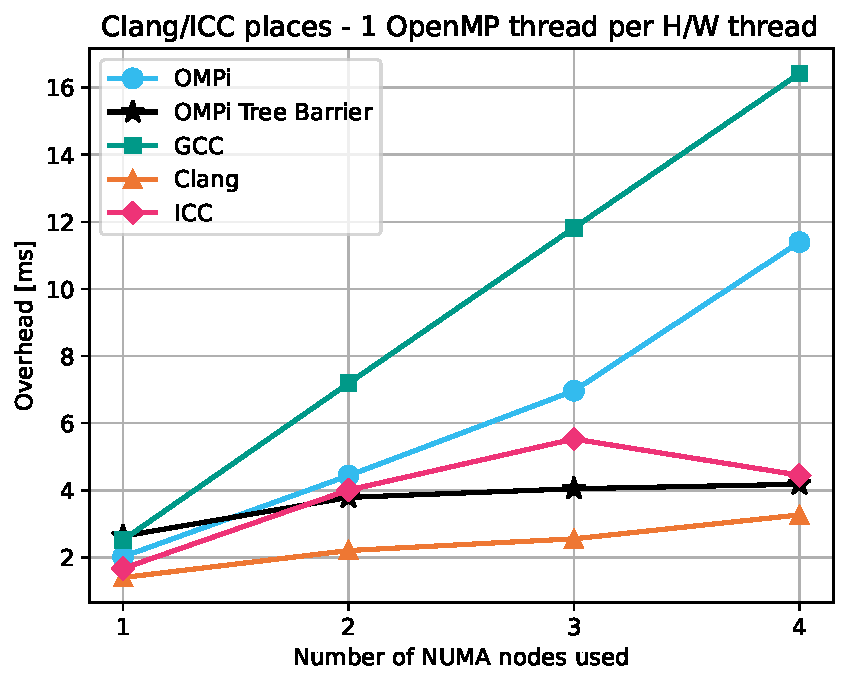
\includegraphics[width=1\textwidth]{Figures/epcc_20210823_175412/clang-places_threads_close.pdf}
        \texttt{OMP\_PLACES=clang-threads}
    \end{minipage}
    \caption{Barrier overhead στον Parade (Clang/ICC places).}
    \label{fig:bo-parade-clang-places}
\end{figure}



\subsubsection{Paragon}
Στα Σχήματα \ref{fig:bo-paragon-default-places} και \ref{fig:bo-paragon-default-places-ompionly} φαίνονται τα αποτελέσματα των μετρήσεων που πραγματοποιήθηκαν στον Paragon. Επειδή κάθε core διαθέτει μόνο ένα H/W thread, τα abstract names \texttt{threads} και \texttt{cores} έχουν το ίδιο αποτέλεσμα. Εξαίρεση αποτελούν οι ICC και Clang οι οποίοι εσφαλμένα θεωρούν ότι κάθε επεξεργαστής διαθέτει ένα μόνο core αντί για δώδεκα, γεγονός που θεωρήθηκε ως σφάλμα (bug) και αγνοήθηκε.

\begin{figure}
    \centering
    \begin{minipage}{0.48\textwidth}
        \centering
        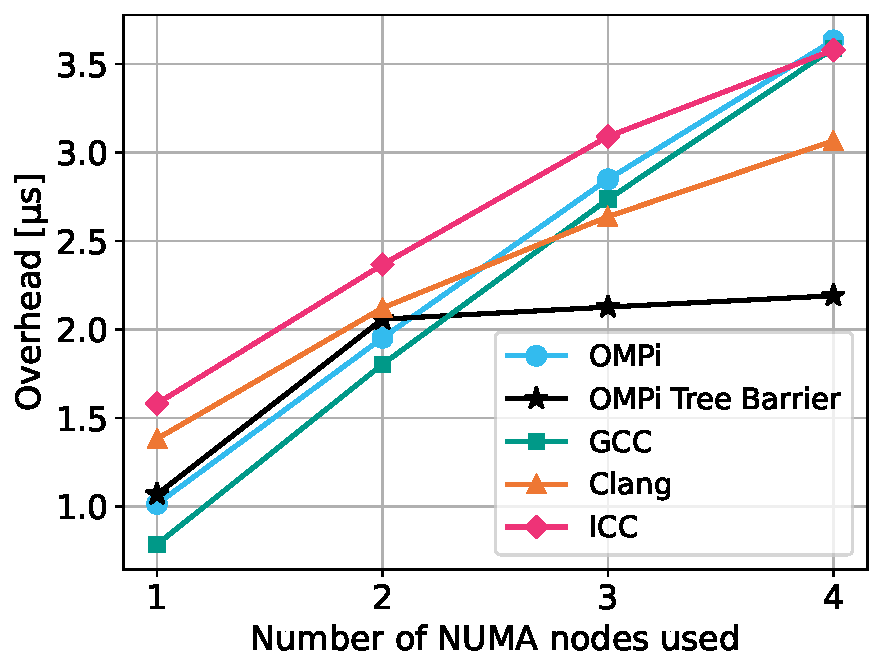
\includegraphics[width=1\textwidth]{Figures/paragon_epcc_20210825_132109/default-places_threads_close.pdf}
		\caption{Barrier overhead στον Paragon.}
		\label{fig:bo-paragon-default-places}
    \end{minipage}\hfill
    \begin{minipage}{0.48\textwidth}
        \centering
        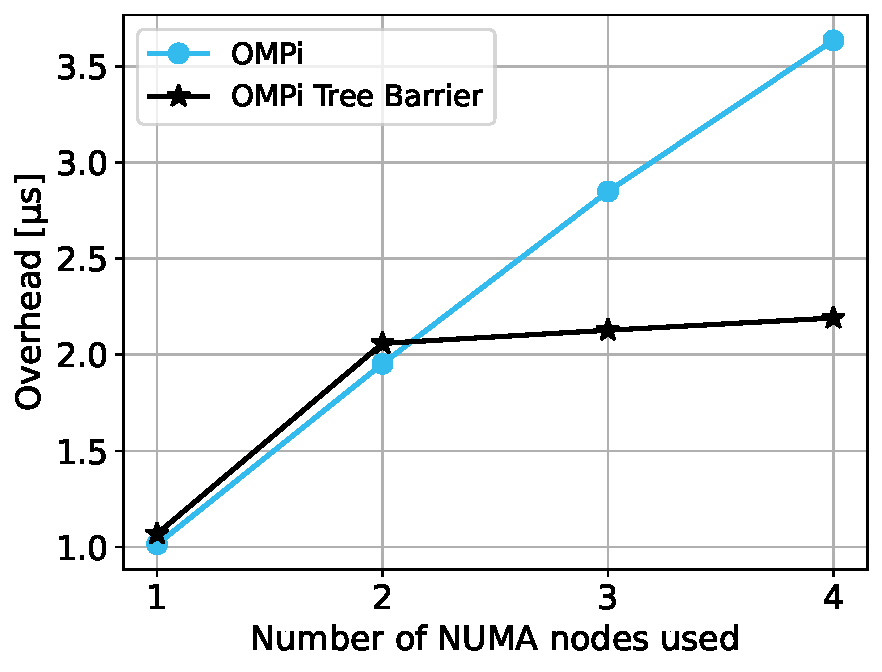
\includegraphics[width=1\textwidth]{Figures/paragon_epcc_20210825_132109/ompi_default-places_threads_close.pdf}
        \caption{Barrier overhead στον Paragon για τους barriers του OMPi.}
        \label{fig:bo-paragon-default-places-ompionly}
    \end{minipage}
\end{figure}


%
%\begin{figure}[t]
%	\centering
%	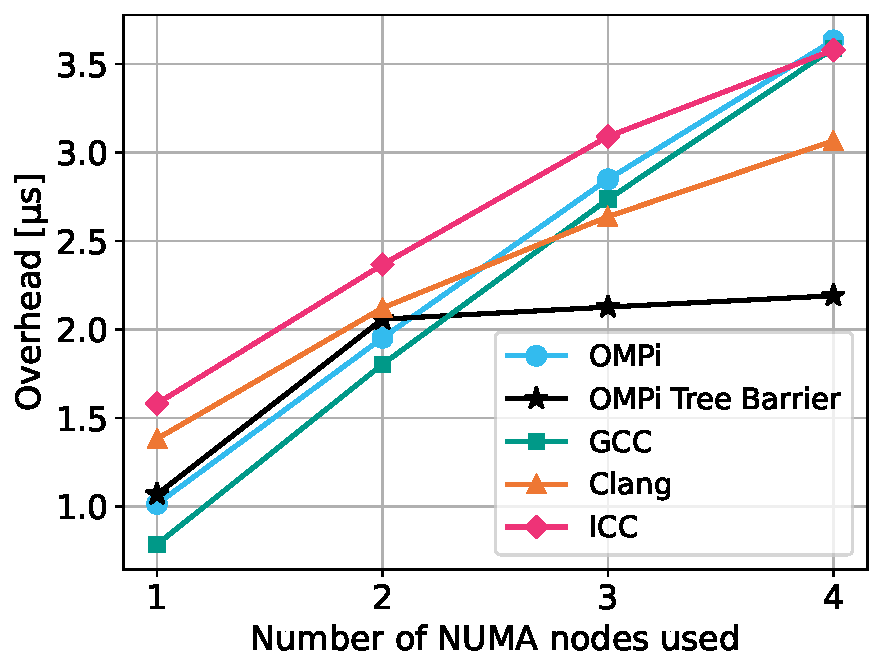
\includegraphics[width=0.7\textwidth]{Figures/paragon_epcc_20210825_132109/default-places_threads_close.pdf}
%	\linebreak
%	\caption{Barrier overhead στον Paragon: OMP\_PLACES=threads.}
%	\label{fig:bo-paragon-threads}
%\end{figure}
%
%\begin{figure}[t]
%	\centering
%	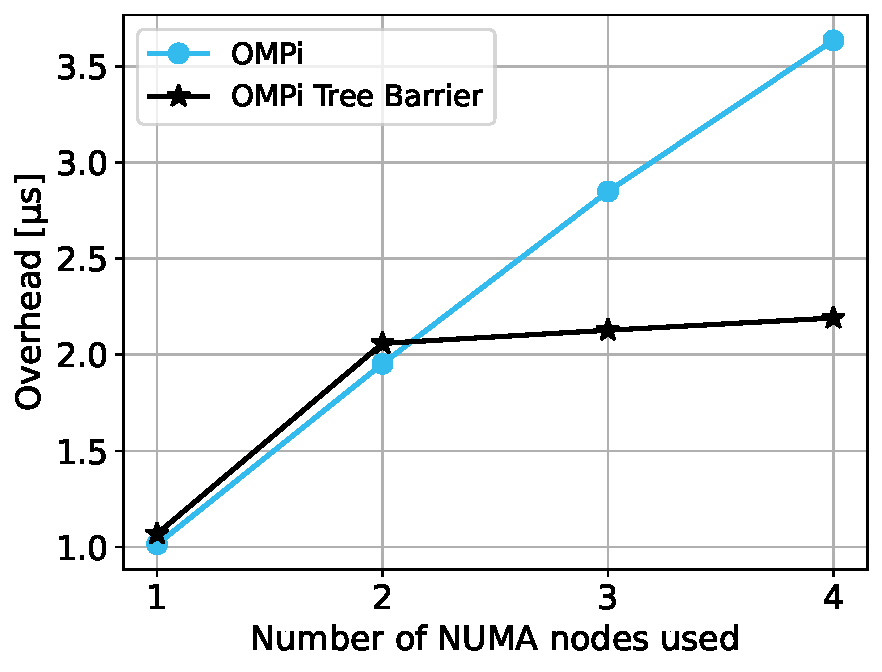
\includegraphics[width=0.7\textwidth]{Figures/paragon_epcc_20210825_132109/ompi_default-places_threads_close.pdf}
%	\linebreak
%	\caption{Barrier overhead στον Paragon για τους barriers του OMPi.}
%	\label{fig:bo-paragon-ompionly}
%\end{figure}

Από τις μετρήσεις στον Paragon παρατηρούμε ότι τα overheads των OMPi, GCC και ICC αυξάνουν σχεδόν γραμμικά και συγκλίνουν για πλήθος τεσσάρων κόμβων. Ο Clang φαίνεται ότι κλιμακώνει καλύτερα για τρεις και τέσσερις κόμβους από τους OMPi, GCC και ICC, αλλά όχι το ίδιο αποδοτικά όπως συνέβαινε στον Parade. Ο OMPi tree barrier επιδεικνύει την καλύτερη επίδοση για τρεις και τέσσερις κόμβους, με το overhead να αυξάνει με πολύ μικρό ρυθμό όσο αυξάνεται το πλήθος των κόμβων, φαινόμενο που παρατηρήθηκε και στον Parade. Επιπλέον, παρατηρούμε ο tree barrier έχει λίγο πιο μεγάλο overhead σε σχέση με τον κλασικό barrier του OMPi, όχι μόνο για ένα κόμβο αλλά και για δύο. Κάτι τέτοιο πιθανώς συμβαίνει καθώς οι δύο κόμβοι ανήκουν στο ίδιο ενσωματωμένο κύκλωμα επεξεργαστή.


\subsubsection{Σύνοψη συμπερασμάτων}
Ο νέος αλγόριθμος tree barrier που υλοποιήθηκε βελτίωσε σημαντικά το κόστος που απαιτεί ο συγχρονισμός των νημάτων όταν χρησιμοποιούνται δύο ή περισσότεροι κόμβοι NUMA, γεγονός που καθιστά εφικτή και αποδοτική την κλιμακωσιμότητα του μεταφραστή OMPi σε συστήματα NUMA πάρα πολλών πυρήνων.


\chapter{Σύνοψη και Μελλοντική Εργασία}

\section{Ανακεφαλαίωση}
Η ανάγκη για όλο και μεγαλύτερη επεξεργαστική ισχύ οδήγησε στη δημιουργία των συστημάτων μη ομοιόμορφης προσπέλασης μνήμης (NUMA), που αποτελούν αρχιτεκτονική εξέλιξη των συμμετρικών πολυεπεξεργαστών (SMPs). Τα συστήματα αυτά παρέχουν κοινόχρηστο χώρο διευθύνσεων και συνεπώς επιτρέπουν τη χρήση διαδεδομένων μοντέλων προγραμματισμού όπως το OpenMP. Λόγω της κατανεμημένης από φυσική άποψη οργάνωση της μνήμης των συστημάτων αυτών, οδηγούμαστε στην εκμετάλλευση πληροφοριών που σχετίζονται με την τοπολογία του υποκείμενου συστήματος για την επίτευξη των βέλτιστων δυνατών επιδόσεων.

Κάτι τέτοιο έρχεται σε αντίθεση με την υψηλού επιπέδου διεπαφή προγραμματισμού εφαρμογών OpenMP, στο πλαίσιο της οποίας χρησιμοποιούνται αφαιρέσεις (abstractions) ώστε να είναι δυνατή η συγγραφή φορητών προγραμμάτων χρήστη. Παρόλα αυτά, λόγω της ανάγκης χρήσης πληροφοριών που σχετίζονται με την τοπολογία του συστήματος, από την έκδοση 4.0 του προτύπου OpenMP και έπειτα, άρχισαν να προδιαγράφονται λειτουργίες που σχετίζονται με την τοπολογία του υποκείμενου συστήματος. Οι λειτουργίες αυτές επιτρέπουν τον ορισμό συνόλων επεξεργαστών (OpenMP places) στα οποία μπορούν να ανατεθούν τα νήματα OpenMP βάσει διάφορων πολιτικών, γνωστών ως OpenMP processor binding policies.

Στα πλαίσια της παρούσας διπλωματικής εργασίας, υλοποιήθηκαν πλήρως τα OpenMP places και OpenMP processor binding policies όπως προδιαγράφονται από την πιο πρόσφατη έκδοση του προτύπου OpenMP και συγκεκριμένα την έκδοση 5.1 (Νοέμβριος 2020). Η ικανότητα ελέγχου του τρόπου ανάθεσης των νημάτων σε σύνολα από επεξεργαστές, επιτρέπει τον διαμοιρασμό των νημάτων στους διαθέσιμους επεξεργαστές ανάλογα με τη λογική οργάνωση της εργασίας που πρέπει να επιτελέσει το πρόγραμμα χρήστη. Επιπλέον, υλοποιήθηκε ένας νέος αλγόριθμος barrier για τον ερευνητικό μεταφραστή OMPi που υποστηρίζει το OpenMP. Σκοπός του νέου αλγορίθμου ήταν η δυνατότητα συγχρονισμού των νημάτων σε συστήματα NUMA με κλιμακώσιμο τρόπο, καθώς το πλήθος των κόμβων αυξάνεται.

Τα μετροπρογράμματα ελέγχου της ορθότητας της υλοποίησης αλλά και μέτρησης του κόστους σε χρόνο (overhead) που απαιτείται για το συγχρονιμό με χρήση barrier, έδειξαν ότι ο νέος barrier έχει τη δυνατότητα να χρησιμοποιείται αποδοτικά για το συγχρονισμό νημάτων που εκτελούνται σε πολλαπλούς κόμβους NUMA. Ιδιαίτερα σημαντικό είναι το γεγονός ότι ο νέος αλγόριθμος barrier σε σχέση με τον κλασικό όχι μόνο είναι λιγότερο κοστοβόρος από άποψη χρόνου, αλλά έχει και καλές ιδιότητες κλιμάκωσης, καθώς για κάθε επιπλέον κόμβο που χρησιμοποιείται, το επιπλέον overhead αυξάνεται με μικρό ρυθμό.

\section{Μελλοντική Εργασία}


% Εισαγωγή της βιβλιογραφίας
\addstarredchapterc{\bibname} % minitoc
\bibliographystyle{IEEEtran}
\bibliography{Content/Bibliography}


% Προαιρετικά, μπορείτε να εισάγετε παραρτήματα
\appendix
\chapter{Τίτλος πρώτου παραρτήματος}
\label{app:FirstAppendix}

Εδώ είναι ο χώρος του πρώτου Παραρτήματος.

\begin{table}[h]
	\centering
	\caption{Πίνακας Παραρτήματος.}
	\label{tab:AppendixTable}
	\begin{tabular}{l l l l l}
		\hline
		~ & ~ & Sample Mean & ~ & 95\% Confidence Interval \\
		\hline
		1 process & ~ & $3.640966$  & ~ & $0.100136$ \\
		4 processes & ~ & $1.053655$  & ~ & $0.037212$ \\
		8 processes & ~ & $0.610223$  & ~ & $0.023470$ \\
		16 processes & ~ & $0.357321$  & ~ & $0.014783$ \\
		32 processes & ~ & $0.227180$  & ~ & $0.016923$ \\
		\hline
	\end{tabular}
\end{table}
\chapter{Η σύνταξη της μεταβλητής περιβάλλοντος OMP\_PLACES}
\label{app:OMP_Places syntax}
Το σύνολο των έγκυρων τιμών που μπορούν να ανατεθούν στη μεταβλητή \texttt{OMP\_PLACES} σύμφωνα με το OpenMP 5.1 \cite{openmp51} προκύπτουν βάσει των ακόλουθων συντακτικών κανόνων:
\begin{verbatim}
	<list>         |= <p-list> | <aname>
	<p-list>       |= <p-interval> | <p-list>,<p-interval>
	<p-interval>   |= <place>:<len>:<stride> | <place>:<len> | <place> | !<place>
	<place>        |= {<res-list>} | <res>
	<res-list>     |= <res-interval> | <res-list>,<res-interval>
	<res-interval> |= <res>:<num-places>:<stride> | <res>:<num-places> | <res>
	                  | !<res>
	<aname>        |= <word>(<num-places>) | <word>
	<word>         |= sockets | cores | ll_caches | numa_domains | threads
	                  | <implementation-defined abstract name>
	<res>          |= non-negative integer
	<num-places>   |= positive integer
	<stride>       |= integer
	<len>          |= positive integer
\end{verbatim}
%\chapter{Τίτλος τρίτου παραρτήματος}
\label{app:ThirdAppendix}

Εδώ είναι ο χώρος του τρίτου Παραρτήματος.

\begin{figure}[h]
	\centering
	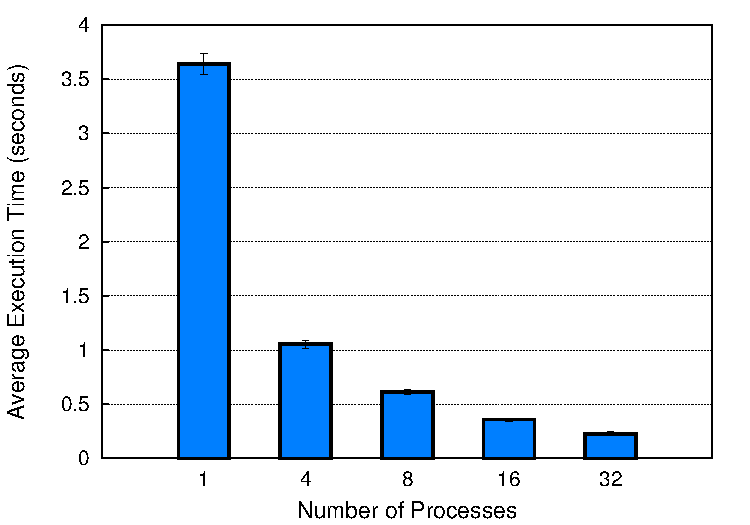
\includegraphics[width=0.65\textwidth]{Figures/MatrixMultiplication.pdf}
	\caption{Εικόνα Παραρτήματος.}
	\label{fig:AppendixFigure}
\end{figure}


% Εκτύπωση του ευρετηρίου (προαιρετικό)
\printindex


\end{document}
